\cotefile{136}
\scanpage{2}
Complexe DR à p.d.

et ombres

\mspage{1}
\scanpage{3}
\mspage{(1)}
Complexe DR à p.d. et ombres des modules.

\margin{Plan conf. IHES en 1976\figure{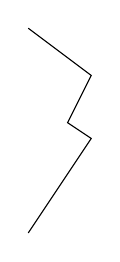
\begin{tikzpicture}\draw (0,2.6)--(.8,2)--(.5,1.4)--(.8,1.2)--(0,0);\end{tikzpicture}}}
\margin{géom. diff.\\ -- anal.\\ -- algébr.\\ \deleted{\unsure{top.}} arithm.\\ top. alg. $\left\{\begin{array}{l}\mathrm{PL}\\ \unsure{\frac12\text{ simpl.}}\end{array}\right.$}

1 Historique

a) Notion des formes diff. (\uline{Poincaré} ?) et formule de \uline{Stokes}
\[
\int_c d\omega=\int_{\partial c}\omega
\qquad(\text{d'où }H^*_{\mathrm{DR}}(X)\longrightarrow H^*(X,\mathbb C))
\]

b) Th. de \uline{De Rham} (conjecturé par \uline{E. Cartan}). \unsure{Mais démonstr.}
\inserted{Maintenant bien compris : th. des faisceaux, lemme Poincaré}

c) Théorie de \uline{Hodge des} intégrales harmoniques
(structure supplémentaire bigraduée sur $H^*_{\mathrm{DR}}(X)$ si $X$ kählérienne compacte)

d) Théorème de \uline{Cartan-Serre} sur variétés de Stein
(ou Lemme de Poincaré valable dans l'analytique \uline{complexe})

e) Cas des variétés algébriques \unsure{ou} schémas, sur corps \unsure{(ou schém. de base finis ?)} : \uline{Dwork}, \uline{Washnitzer} -- \uline{Monsky}, plus tard le yoga ``cristallin'' développé par \uline{Berthelot}, \uline{Illusie}, \deleted{\unsure{et différents}} \inserted{\uline{Messing}, Mazur} \deleted{\unsure{autres}}. \margin{avec Hartshorne, Herrera, Ogus, Bloch (!)} Ici on trouve des théories coh. qui ne sont plus à ``anneau de coeff'' de car. nulle i.e. contenant $\mathbb Q$ -- \unsure{i.e.} en principe les phénomènes de torsion ne sont pas perdus.
\inserted{Du pt de vue Weil, c'était un défaut impardonnable !}

f) Th. de \uline{Grothendieck} pour variétés algébriques sur $\mathbb C$ (\deleted{\unsure{généralisé}} \inserted{\uline{généralisé}} par \uline{Deligne}, \uline{Hartshorne} pour des coeff plus généraux) Ceci donne \unsure{un sens} (au moins en car. 0) à la \uline{signification} topologique de la coh. de De Rham ``\uline{algébrique}'' des schémas algébriques.

g) Complexe de De-Rham-Sullivan pour espaces topologiques généraux : \uline{formes différentielles singulières} $C^\infty$ \deleted{\unsure{\mathbb C}\unsure{-alg. resp.}} $\mathbb C$-algébrique, resp. $\mathbb R$-algébrique resp. $\mathbb Q$-algébrique). Donne la coh. à coeff dans $\mathbb C$ (resp. $\mathbb R$, resp. $\mathbb Q$) (facile). Sullivan montre même

\margin{\diagram{\begin{tikzcd}
C^\bullet_{\mathrm{DRS}\,\mathbb R\text{-alg}} \arrow[r,phantom,"\unsure{\subset}" description] & C^\bullet_{\mathrm{DRS}\,C^\infty} \arrow[r,phantom,"\subset" description] \arrow[d,phantom,"\cup" description] & C^\bullet_{\mathrm{DRS}} \\
\deleted{\unsure{C}} & C^\bullet_{\mathrm{DR}} &
\end{tikzcd}}}
\mspage{2}
\scanpage{4}
\mspage{(2)}
que le $\mathbb Q$-type d'homotopie de $X$ est récupéré si $X$ est simplement connexe (\uline{sauf erreur}) -- de façon plus précise, il y a une équivalence de cat. \inserted{\unsure{donnée} par $C^{\unsure{*}}_{\mathrm{DRS}}$} entre la cat. hom. \inserted{faible} des espaces connexes et simplement connexes (du pt de vue singulier), et une certaine catégorie dérivée formée avec les $\mathbb Q$-algèbres graduées associatives et \inserted{anti} comm. \deleted{telles} à degrés $\geq 0$ telles que
\[
H^0(A)\simeq\mathbb Q\quad \deleted{\unsure{H^0(A)\simeq0}}\quad H^1(A)\simeq0.
\]
Il y a une théorie des modèles minimaux \inserted{pour de telles algèbres}, une façon très simple de récupérer les $\pi_i\otimes_{\mathbb Z}\mathbb Q$ en fonction d'un tel modèle... (On renvoie aux papiers de Sullivan)

Mais à nouveau, -- \unsure{perd} la torsion !

\figure{\begin{tikzpicture}\draw (0,0)--(14,0);\end{tikzpicture}}

Dém. du th. d'isomorphie de Sullivan
\[
H^q(C^\bullet_{\mathrm{DRS}\unsure{/\mathbb Q}}(X,\mathbb Q))\simeq H^q(X,\mathbb Q).
\]

$\forall n\geq0$, $[n]$ simplexe type de dim $n$

$\Delta^{[n]}_{\unsure{\mathbb R|*}}$ sa réalisation géométrique.
\margin{$(\sum_0^n X_i=1,\ \unsure{\forall}X_i\geq0)$}

$E^{[n]}$ l'espace affine qu'il sous-tend (avec une $\mathbb Q$-structure)
\margin{$\sum_0^n X_i=1$ dans $\mathbb R^{n+1}$}

$\unsure{\mathrm{DRS}^\bullet_{[n]}}=\unsure{C^\bullet_{\mathbb Q\mathrm{DR}}}(E^{[n]})$ son complexe de De Rh. -- $\mathbb Q$-algébrique.

C'est contravariant en $[n]$, d'où
\[
\mathrm{DRS}^\bullet_*=(\mathrm{DRS}_{[n]})_{n\geq0}
\]
Algèbre différentielle graduée \deleted{\unsure{semi}}\inserted{semi}-simpliciale (et $=$ simpliciale) -- à degrés $\geq0$, anticommutative.

Pour tt espace topologique $X$, $S_*(X)$ son complexe singulier $\frac12$ simplicial. On a
\[
C^\bullet_{\mathrm{DRS}}(X,\mathbb Q)\simeq\operatorname{Hom}(\unsure{S_*(X)},\mathrm{DRS}^\bullet_*)
\]
\mspage{3}
\scanpage{5}
\mspage{(3)}
i.e. a) $C^\bullet_{\mathrm{DRS}}(X,\mathbb Q)$ dépend de $X$ via $S_*(X)$

b) Sur $(\mathrm{Ss}\unsure{\simeq}(\mathrm{Ens})_*$, le foncteur $C^\bullet_{\mathrm{DRS}}(-,\mathbb Q)$ est représentable par $\mathrm{DRS}^\bullet_*$.

Or a) $\mathrm{DRS}^\bullet_*$ est une résolution de $\mathbb Q_*$ \inserted{(dans la cat. des groupes $\frac12$ simpl.)} (lemme de Poincaré algébrique sur les espaces \inserted{$\mathbb Q$-}affines $E^{[n]}$)

b) Les composantes $\mathrm{DRS}^i_*$ $(i\geq0)$ de $\mathrm{DRS}^\bullet_*$ sont des objets \inserted{acycliques} du topos $\mathrm{Ss}$ (ce qui revient à dire que leurs $\pi_j(\mathrm{DRS}^i_*)$ sont nuls, ce qui se vérifie facilement). [\unsure{Il en serait itou} avec des formes $C^\infty$ à coeff dans $\mathbb R$ ou $\mathbb C$, -- analytiques réelles, ou analytiques complexes...]

\deleted{\unsure{On peut prendre}}\figure{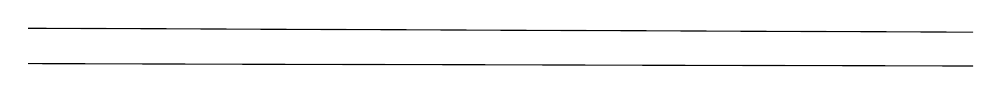
\begin{tikzpicture}\draw (0,.45)--(12,.4);\draw (0,0)--(12,-.03);\end{tikzpicture}}
\margin{On aimerait avoir une $\mathbb Z$-algèbre diff. $C^\bullet_{\mathrm{DR}}(X,\mathbb Z)$ \uline{\unsure{anticomm.}} (dépendant fonct. de $X$ par $S_*(X)$) dont la coh. soit la coh. \unsure{entière de $X$|entière avec $\mathbb Z$}. Mais il paraît qu'il y a des ths contre ! On va pourtant y arriver \deleted{\illegible{1}} \inserted{\unsure{quand même !|en un sens !}}}

Si on prend $C^\bullet_{\mathbb Z\text{-}\mathrm{DR}}(E^{[n]})$ (car $E^{[n]}$ a une $\mathbb Z$-structure affine) c'est a) qui devient déjà faux : pour intégrer $\int x^n\,dx$, il faut un dénominateur \inserted{avec $\dfrac{x^{n+1}}{n+1}$} ! Mais en géom. alg. on est déjà familiarisé avec une façon de sauter à pieds-joints \deleted{sur} \inserted{par dessus} le \unsure{caniveau}, en introduisant des p.d. et des polynômes \inserted{(ou séries formelles)} à puiss. div. Si $E^{[n]}$ avait une origine sur $\mathbb Z$ (i.e. provenant \unsure{can.} d'un $\mathbb Z$-module libre de t.f.) -- on aurait un complexe de De Rham à p.d. Mais pas pour un espace affine ! Notons
\[
\begin{aligned}
\mathrm{DRS}^\bullet_{[n]}&\simeq\deleted{\mathbb Q[X_i,dX_i]/}\ C^\bullet_{\mathrm{DR}/\mathbb Q}\left(\mathbb Q[(X_i)_{0\leq i\leq n}]/\textstyle\sum X_i-1\right)\\
&\simeq\mathbb Q[X_i,dX_i]_{0\leq i\leq n}/(\textstyle\sum X_i-1,\ \sum dX_i)\\
&\simeq\mathbb Q[X_0,\ldots,X_{n-1}][dX_0,\ldots,dX_{n-1}]
\end{aligned}
\]
\mspage{4}
\scanpage{6}
\mspage{(4)}
Donc on aurait envie de prendre
\[
\deleted{\mathbb Q}\ \mathbb Z(\{X_i\}[dX_i])_{0\leq i\leq n}/(\textstyle\sum X_i-1,\sum dX_i)_{\mathrm{pd}}
\]
où $\{\ \}$ désigne les pol. à p.d., mais ce n'est plus
\[
\simeq\mathbb Z\{X_0,\ldots,X_{n-1}\}[dX_0,\ldots,dX_{n-1}]
\]
(\deleted{qui est} \inserted{bien} \deleted{qui est} une résolution de $\mathbb Z$), car si on veut tirer de la relation $\sum_0^n X_i-1=0$,
\[
X_n=1-\sum_0^{n-1}X_i\quad
(\inserted{\text{et}}\ dX_n=-\sum_0^{n-1}dX_i\ \text{de }\sum_{\unsure{1}}^n dX_i=0)
\]
-- on a le ``\unsure{hic|bec}'' que $1-\sum_0^{n-1}X_i$ n'appartient pas à l'idéal à p.d. donné dans $\mathbb Z\{X_0,\ldots,X_{n-1}\}$ (donc on ne sait pas comment envoyer $\mathbb Z\{X_0,\ldots,X_{\unsure{n-1|n}}\}$ dans $\mathbb Z\{X_0,\ldots,X_{n-1}\}$ avec \unsure{même} \deleted{\unsure{noyau}} $\sum_0^n X_i-1$ dans le noyau....).

On s'en tire en prenant un anneau de coeff. différent de $\mathbb Z$, soit $S$, avec une \deleted{indéterminée} \inserted{``paramètre''} $t\in S$ fixé dont on \uline{sache prendre des p.d.} \inserted{(i.e. $t\in J$, $J$ idéal à p.d. de $S$)}, et en remplaçant les équations $\sum X_i=1$ de $E^{[n]}$ par l'équation
\[
\sum X_i=t\qquad\text{dans }S^{n+1}
\]
et définissant
\[
\unsure{(C^\bullet_{\mathrm{DRpd}\,t_{[n]}}(S,t))}=\left(S\{X_i\}_{0\leq i\leq n}[dX_i]_{0\leq i\leq n}\right)/(\textstyle\sum X_i-t,\sum dX_i)_{\mathrm{pd}}
\]
(On divise par l'\uline{idéal à p.d.} engendré par $\sum X_i-t$, $\sum dX_i$, ce qui a un sens
\mspage{5}
\scanpage{7}
\mspage{(5)}
car dans $S\{X_i\}[dX_i]$ l'idéal formé des formes \inserted{à p.d.} d'augmentation $\in J$ est à p.d.
\[
\left(S\{X_i\}_{0\leq i\leq n}/(\textstyle\sum X_i-t)_{\mathrm{pd}}\right)\otimes_S\bigwedge^*\left(S^{[n]}/\operatorname{diag}\unsure{S^{[n]}}\right)
\]
C'est une $S$-algèbre diff. \inserted{graduée} anti comm., à degrés $\geq0$, \inserted{augmentée vers $S/J$} à p.d. sur l'idéal \deleted{engendré par $\bigwedge^+$, $S\{X_i\}^+$ et $J\{X_i\}$ \unsure{dans le premier}} l'idéal noyau de l'augmentation
\[
C^\bullet_{\mathrm{DRpd}\,[n]}(S,J,t)\longrightarrow S/J\ ;
\]
\margin{la diff est compatible avec les p.d. i.e. $d(x^{(n)})=x^{(n-1)}dx$}
et comme telle isomorphe à $S\{X_0,\ldots,X_{n-1}\}[dX_0,\ldots,dX_{n-1}]$ qui \uline{est une résolution de $S$}.
\deleted{Donc a) est acquis. Mais faute de b), on ne peut dire a priori ce \unsure{(et il ne sera)} que fait $H^{\unsure{q}}C^\bullet$.}
Pour $[n]$ variable, on trouve
\[
C^\bullet_{\mathrm{DRpd}\,*}{}^{(S,J,t)}=\left(C^\bullet_{\mathrm{DRpd}\,[n]}{}^{(S,J,t)}\right)_{n\geq0}
\]
qui est une rés. $\frac12$ simpliciale (et $=$ simpliciale) de $S$, \inserted{avec aug. vers $S/J=k$, et p.d. sur l'idéal d'augm., comp. à d}. Elle dépend fonctoriellement de $(S,J,t)$, et elle permet de former, \inserted{pour $\mathcal X_*\in(\mathrm{Ss})$}
\[
C^\bullet_{\mathrm{DRpd}}(\mathcal X_*;S,J,t)=\operatorname{Hom}(\mathcal X_*,C^\bullet_{\mathrm{DRpd}\,*}(S,J,t))
\]
foncteur contravariant en $\mathcal X_*$ ! (et si $X$ esp. top.
\[
\begin{aligned}
C^\bullet_{\mathrm{DRpd}}(X;\quad)&=C^\bullet_{\mathrm{DRpd}}(S_*(X);\text{---})\\
&=\operatorname{Hom}(\unsure{C_*(X)|\mathbb Z_*(X)},C^\bullet_{\mathrm{DRpd}\,*}(\quad))
\end{aligned}
\]
\margin{à valeurs dans les $\unsure{S}$-algèbres graduées diff. $S/J$-augmentées, à p.d. sur l'idéal d'augmentation, compatibles avec la diff.}
Mais on ne peut dire en général quelle est sa cohomologie, \inserted{(on a seulement $H^{\unsure{\bullet|0}}_{\mathrm{DRpd}}(\mathcal X_*;S,J,t)\longrightarrow H^{\unsure{\bullet|0}}(\mathcal X_*,S)$)} et en tous cas elle ne sera pas isom. (pour $\mathcal X_*$ variable) à $H^\bullet(\mathcal X_*,S)$.
\mspage{6}
\scanpage{8}
\mspage{(6)}
\inserted{Mais}
Soit $k$ anneau comm. (\unsure{com. unit.}) et $T$ une indéterminée, on prendra dorénavant
\[
S=k\{T\},\quad J=k\{T\}^+=\operatorname{Ker}(k\{T\}\unsure{-|\longrightarrow}k)
\qquad t=T.
\]
Donc
\[
\left\{\begin{aligned}
C^\bullet_{\mathrm{DRpd}\,[n]}{}^{(S,J,t)}&\simeq
\underbrace{k\{T,X_0,\ldots,X_n\}/(\textstyle\sum X_i-T)_{\mathrm{pd}}}_{\displaystyle\simeq\ k\{X_0,\ldots,X_n\}}
\otimes_k\bigwedge^\bullet k^{[n]}/k\\
S/J&\simeq k
\end{aligned}\right.
\]
Soit
\diagram{\begin{tikzcd}[column sep=large]
\Phi_{k*}=\bigl[[n]\mapsto k^{[n]}\bigr]\arrow[r,"\text{inclusion diagonale}"'] & k_*=([n]\mathbin{-}k)
\end{tikzcd}}
\[
\Psi_{k*}=\Phi_{k*}/(k_*)=([n]\mathbin{-}k^{[n]}/\underbrace{k}_{\mathrm{diag}})
\]
On a alors
\[
\begin{array}{c}
C^\bullet_{\mathrm{DRpd}\,*}(k\{T\},k\{T\}^+,\unsure{k|T})\simeq\Gamma^\bullet_k\Phi_{k*}\otimes_k\bigwedge^\bullet\Psi_{k*}\\
\Vert\ \mathrm{dfn}\\
C^{\bullet\bullet}_{\mathrm{DRpd}\,*}(k)
\end{array}
\]
\[
\boxed{C^{\bullet\bullet}_{\mathrm{DRpd}\,*}(k)\simeq\Gamma^\bullet_k\Phi_{k*}\otimes_k\bigwedge^\bullet\Psi_{k*}}
\]
\uline{Structure} : \inserted{$k\{T\}$-}Algèbre \deleted{\unsure{diff.}} \uline{bigraduée} (deg. \unsure{complém.} \uline{et} degré extérieur, d'où degré total) \inserted{unit.} assoc. \deleted{anticomm.} \uline{alternée} (anticomm. $+$ carré des éléments de degré impair nuls), augmentée vers $k$, à p.d. sur l'idéal d'augm., avec diff de bidegré $-1,+1$ (donc degré total 0) \inserted{compatible aux p.d.}
\margin{La bigraduation provient de la gr. \uline{entière} de $S$, et \unsure{du degré ext.} (\unsure{est homogène}) (i.e. de degré 1)}
\mspage{7}
\scanpage{9}
\mspage{(7)}
\uline{Ces structures sont héritées par les}
\[
\boxed{\begin{aligned}
C^{\bullet\bullet}_{\mathrm{DRpd}}(\mathcal X_*,k)&\overset{\mathrm{dfn}}=C^\bullet_{\mathrm{DRpd}}(\mathcal X_*;k\{T\},k\{T\}^+,T)\\
&=\operatorname{Hom}(\mathcal X_*,C^{\bullet\bullet}_{\mathrm{DRpd}\,*}(k))
\end{aligned}}
\]
et dépendent de façon contravariante de $\mathcal X_*$, (covariante de $k$).

$\Phi_{k*}$ est \deleted{\unsure{?}} \inserted{un $k$-Module $\frac12$ simplicial} homotope à 0 donc $\Gamma^p_k(\Phi_{k*})\otimes\bigwedge^q\Psi_{k*}$ \deleted{\unsure{est}} est homotope à $\Gamma^p_k(0)\otimes\bigwedge^q\Psi_{k*}$, donc hom. à 0 si $p\ne0$.

Donc $C^{p,q}_{\mathrm{DRpd}\,*}(k)$ est hom. à 0 (donc \deleted{flasque} \inserted{acyclique}) si $p=0$. En degré total donné \inserted{$n$}, on a
\diagram{\begin{tikzcd}[column sep=small]
0\arrow[r] & C_*^{n,0}\arrow[r] & C_*^{n-1,1}\arrow[r] & C_*^{n-2,2}\arrow[r,dash] & \cdots & C_*^{\unsure{1},n-1} & C_*^{0,n}\arrow[l]\arrow[r] & 0\arrow[d]\\
& k_*\arrow[u] & & & & & &0\arrow[d]\\
& & & & & & &0
\end{tikzcd}}
i.e. on trouve une résolution \deleted{flasque} \inserted{de long. $n$} de $k_*$ par des \deleted{groupes} \inserted{$k$-Modules} $\frac12$ simpliciaux qui sont acycliques sauf le dernier -- donc on peut la considérer comme une tronquée en l'\deleted{indice} \inserted{degré} $n$ d'une résolution flasque de $k_*$ -- la cohomologie de ses sections sur un $\mathcal X_*$ est donc la coh. de $\mathcal X_*$ tronquée en degré $n$ :
\[
H^{p,q}_{\mathrm{DRpd}}(\mathcal X_*,k)\simeq
\begin{cases}
H^q(\mathcal X_*,k)&\text{si }q\leq p+q\ \text{i.e. }p\geq0\\
0&\text{si }p<0
\end{cases}
\]
\mspage{8}
\scanpage{10}
\mspage{(8)}
Mais quelle est \inserted{(pour $q$ fixé)} la structure de $k\{T\}$-module de $H^{\bullet,q}_{\mathrm{DRpd}}(\mathcal X_*,k)$ ? \deleted{On voit que} pour le \uline{degré total} (égal au degré \unsure{extérieur} : \uline{plus} $q$) on trouve $H^0(\mathcal X_*,k)\otimes_k k\{T\}$ tronqué en degrés $\geq q$, donc
\[
H^{\bullet,q}_{\mathrm{DRpd}}(\mathcal X_*,k)\simeq\tau_q\left(H^0(\mathcal X_*,k)\otimes_k k\{T\}\right)[q]
\]
\margin{(translation des degrés par $-q$)}

Si on réindexe les bidegrés par le couple (degré total, degré extérieur)
\[
H'^{n,q}_{\mathrm{DRpd}}(\mathcal X_*,k)=H^{\overbrace{n-q}^{p},q}_{\mathrm{DRpd}}(\mathcal X_*,k)
\]
(donc la condition de degré $p,q\geq0$ devient $n\geq q\geq0$, l'op. diff est de bidegré $(0,1)$ donc c'est un hom (\uline{homogène}) de $S$-modules gradués), on trouve
\[
H'^{\bullet,q}_{\mathrm{DRpd}}(\mathcal X_*,k)\simeq\tau_q\left(H^q(\mathcal X_*,k)\otimes_k k\{T\}\right)
\]
Ces isom. sont compatibles avec les structures multiplicatives (et bien entendu fonctoriels en $\mathcal X_*,k$...). Donc \inserted{\uline{a priori}} on ne récupère pas \inserted{(via $H'^{\bullet\bullet}_{\mathrm{DRpd}}(\mathcal X_*,k)$)} les $k$-modules $H^q(\mathcal X_*,k)$ et leurs \inserted{cup-}accouplements, mais les $k$-modules \inserted{gradués} $\tau_q(H^q(\mathcal X_*,k)\otimes_k k\{T\})$ et leurs accouplements déduits du cup des $H^\bullet(\mathcal X_*,k)$.
\mspage{9}
\scanpage{11}
\mspage{(9)}
Ce qui donne à penser que le complexe de DR. p.d. de $\mathcal X_*$ \inserted{à coeff dans $\mathbb Z$ disons} (même dans le cas $k=\mathbb Q$ qu'il contient) donne \unsure{une} information homotopique précise sur $\mathcal X_*$, c'est l'observation qu'en fait, pour un \deleted{module gradué} $k$-module $M$ quelconque, on récupère $M$ à isom canonique près par la connaissance d'un quelconque des tronqués $\tau_q(M\otimes_k S)$ \inserted{\unsure{qu'on appelle|j'appelle} la \uline{$q$ième ombre de $M$}} (quelque grand que soit $\unsure{p|q}\ldots$), et de $=$ l'accouplement $M\otimes N\mathbin{-}P$ est connu quand on connaît, pour $q$ assez grand, l'accouplement correspondant $\tau_q(M_S)\otimes\tau_q(N_S)\mathbin{-}\tau_q(P_S)$.

Donc une \inserted{$k$-}algèbre graduée $H^\bullet$ à degrés $\geq0$ \deleted{est} est connue à isom canonique près quand on connaît la $S$-algèbre bigraduée dont les composantes \inserted{de degré} ``extérieur'' \inserted{$q$} sont les $\tau_q(H^q\otimes_k S)$.... \deleted{Ainsi} Cette ``théorie des ombres'' étant \inserted{\unsure{supposée}} acquise, on voit que la connaissance de $C^{\bullet\bullet}_{\mathrm{DRpd}}(\mathcal X_*,k)$ \inserted{(en tant que $S$-algèbre diff. bigraduée)} implique celle de l'algèbre graduée $H^\bullet(\mathcal X_*,k)$ -- et en raffinant un peu, on \inserted{voit que} $\unsure{F|\vDash}\ R^\bullet\Gamma(\mathcal X_*,k)$ comme objet de la cat. dérivée $D(k)$, \uline{plus} l'accouple-
\mspage{10}
\scanpage{12}
\mspage{(10)}
ment de cup-produit
\[
R\Gamma(\mathcal X_*,k)\overset{L}{\otimes}R\Gamma(\mathcal X_*,k)\mathbin{-}R\Gamma(\mathcal X_*,k)
\]

\uline{\unsure{Remarques|Remarque} et Pbs}

a) Si $k$ est une $\mathbb Q$-algèbre, de sorte que $C^\bullet_{\mathrm{DRS}}(\mathcal X_*,k)$ est défini, on le reconstruit à partir de $C^{\bullet\bullet}_{\mathrm{DRpd}}(\mathcal X_*,k)$ \deleted{\unsure{comme}} par la formule
\[
C^\bullet_{\mathrm{DRS}}(\mathcal X_*,k)\simeq C^{\bullet\bullet}_{\mathrm{DRpd}}(\mathcal X_*,k)/(T-1)
\]
Plus généralement, \uline{quelque soit} $k$, on a
\[
C^\bullet_{\mathrm{DRS}}(\mathcal X_*,\underbrace{k\otimes_{\mathbb Z}\mathbb Q}_{k_{\mathbb Q}})\simeq C^{\bullet\bullet}_{\mathrm{DRpd}}(\mathcal X_*,k)/(T-1)
\]
[Et plus gén. encore, si $(S,J,t)$ comme au début
\[
C^\bullet_{\mathrm{DRpd}}(\mathcal X_*;S,J,t)/(t-1)\simeq C^\bullet_{\mathrm{DRS}}(\mathcal X_*,S_{\mathbb Q}/(t-1))
\]
]
\margin{?}

b) Je suis convaincu que la structure à p.d. sur l'idéal d'augmentation de
\[
C^{\bullet\bullet}_{\mathrm{DRpd}}(\mathcal X_*,k)\mathbin{-}H^{\unsure{0|q}}(\mathcal X_*,k)=\operatorname{Hom}(\mathcal X_*,k_*)
\]
est importante. \deleted{\unsure{Il n'est peut-être pas}} l'idée de se poser la question, pour $\mathcal X_*$ simplement connexe, \margin{avec conditions de finitude sur $\mathcal X_*$, disons les $H_i(\mathcal X_*)$ de t.f.} si la connaissance de $C^{\bullet\bullet}_{\mathrm{DRpd}}(\mathcal X_*,k)$ \uline{avec ttes ses structures} (y compris celles des p.d.) n'implique pas la connaissance du type d'homotopie de $\mathcal X_*$. On peut
\mspage{11}
\scanpage{13}
\mspage{(11)}

plus précisément appeler \uline{complexe de De Rham à p.d. virtuel} \inserted{\uline{sur $k$}} \deleted{\unsure{un} complexe de} $k$-bi-algèbre diff. \unsure{augmentée}, ass. unit. alternée, à diff de bidegré $-1,+1$ \deleted{(ou $0,+1$ au choix)} à bidegrés $\geq 0$, avec p.d. sur l'idéal d'augm., compatibles avec la diff $(d(x^{(n)})=x^{(n-1)}dx)$, et telle que les $H^{\bullet,q}(C^{\bullet\bullet})[-q]$ soient des $q$-ombres\unsure{?} (auquel cas on récupère à partir de $C^{\bullet\bullet}$ un élément de $D(k)$ avec structure multiplicative ass. unit. comm.\dots), passer à une ``catégorie dérivée'' de ces complexes en ``inversant'' les flèches qui sont des \unsure{qu-isom}, d'où par $C^{\bullet\bullet}_{\mathrm{DRpd}}(\mathcal X_\bullet,k)$ un foncteur
\diagram{\begin{tikzcd}[column sep=large]
\begin{array}{c}(\mathrm{Hot})\\ \text{types d'hom}\end{array}
\arrow[r] &
\begin{array}{c}(\mathrm{DRpd})\\ \text{cat. dérivée}\\ \text{des complexes}\\ \mathrm{DRpd}\end{array}
\end{tikzcd}}
et on peut se demander si sa restriction aux espaces connexes et simplement connexes avec des $H^i_{\unsure{*}}(X,\mathbb Z)$ de t.f. (cas $k=\mathbb Z$) \deleted{est} \inserted{induit} une équivalence avec les complexes de DRàpd sur $\mathbb Z$ tels que $H^0(C^{\bullet\bullet})\simeq k$, $H^1(C^{\bullet\bullet})=0$, les $H^i(C^{\bullet\bullet})$ de t.f. sur $\mathbb Z$\dots

\mspage{12}
\scanpage{14}
\mspage{(12)}

c) J'ai un peu réfléchi \deleted{\unsure{aux}} si on peut reconstruire les op. coh. \deleted{\unsure{dans}} (type Steenrod ou Whitney) dans la coh. de $\mathcal X_*$ par la connaissance de $C^{\bullet\bullet}_{\mathrm{DRpd}}(\mathcal X_*,-)$, et n'ai que des résultats \inserted{partiels} négatifs qui montrent qu'avec des \unsure{auto} multiplicatifs de $C^{\bullet\bullet}_{\mathrm{DRpd}*}(\deleted{\mathbb Z}\inserted{k})$ on ne trouve rien d'intéressant.

d) Il faudrait sans doute donner des modèles minimaux à la Sullivan, pour essayer entre autres d'exprimer \unsure{les} groupes d'homotopie de $\mathcal X_*$ en termes de $C^{\bullet\bullet}_{\mathrm{DRpd}*}(\mathcal X_*,\mathbb Z)$ (cas où $\mathcal X_*$ \deleted{\unsure{simplt}} connexe avec cond. de finitude\dots) Je n'ai rien fait dans cette direction. Je n'ai $=$ pas développé une formule de Künneth pour $C^{\bullet\bullet}_{\mathrm{DRpd}}$ d'un produit $\mathcal X_*\times\mathcal Y_*$ -- il y a des difficultés techniques dues au fait qu'on ne peut sans doute supposer $C^{\bullet\bullet}_{\mathrm{DRpd}}(\mathcal X_*\text{ ou }\mathcal Y_*,k)$ \unsure{plats} sur $k\{T\}$.

\mspage{13}
\scanpage{15}
\mspage{(13)}

e) Le complexe de chaines $C_\bullet(\mathcal X_*,\deleted{\mathbb Z}\inserted{k})$ permet de reconstruire tous les complexes de cochaines $C^\bullet(\mathcal X_*,k')$, pour $k'$ \inserted{$k$-Alg.} variable, par
\[
C^\bullet(\mathcal X_*,k)\simeq\operatorname{Hom}_{\mathbb Z}(C_\bullet(\mathcal X_*,\deleted{\mathbb Z}\inserted{k}),k).
\]
\inserted{(L'objet ``le plus fin'' est le $C_\bullet(\mathcal X_*,\mathbb Z)$, on a donc $C_\bullet(\mathcal X_*,k)\simeq C_\bullet(\mathcal X_*,\mathbb Z)\otimes_{\mathbb Z}k$)}
Il est possible de même de définir une \unsure{cobigèbre} \inserted{diff} $C_{\bullet\bullet}^{\mathrm{DRpd}}(\mathcal X_*,\deleted{\mathbb Z}\inserted{k})$ \inserted{$k$-coaugmentée} à copuiss. div., telle que l'on ait, pour $\forall$ $k$-Alg. $k'$ :
\[
C^{\bullet\bullet}_{\mathrm{DRpd}}(\mathcal X_*,k')\simeq\operatorname{Hom}_k(C_{\bullet\bullet}^{\mathrm{DRpd}}(\mathcal X_*,k),k')
\]
(compatible avec \unsure{ttes} les structures).

On aura d'ailleurs
\[
C_{\bullet\bullet}^{\mathrm{DRpd}}(\mathcal X_*,k')\simeq C_{\bullet\bullet}^{\mathrm{DRpd}}(\mathcal X_*,k)\otimes_k k'.
\]
L'objet le plus fin est $C_{\bullet\bullet}^{\mathrm{DRpd}}(\mathcal X_*,\mathbb Z)$. C'est lui qu'il convient de considérer (au lieu de son ``dual'' $C^{\bullet\bullet}_{\mathrm{DRpd}}(\mathcal X_*,\mathbb Z)$) si on veut aborder b) c) d) sans condts de finitude.

Notons que [\unsure{$\forall$ comme|tt comme} $C^{\unsure{*|\bullet\bullet}}_{\mathrm{DRpd}}(\mathcal X_*,k)$, pour $\mathcal X_*$ variable, transforme $\varinjlim$ quelconq. en $\varprojlim$] $C_{\bullet\bullet}^{\mathrm{DRpd}}(\mathcal X_*,\mathbb Z)$ \deleted{transforme} \inserted{commute aux} $\varinjlim$ quelconques (pas néc. \unsure{filtrantes}).

\mspage{14}
\scanpage{16}
\mspage{14}

\margin{\figure{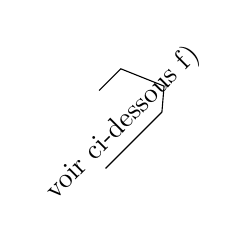
\begin{tikzpicture}[x=0.55cm,y=0.55cm]\draw (0,1.8)--(.5,2.3)--(1.5,1.9)--(1.45,1.3)--(.15,0);\node[rotate=45] at (.55,1.05) {\uline{voir ci-dessous \unsure{f)}}};\end{tikzpicture}}}
\deleted{\unsure{f)}}\inserted{\unsure{g)}} \uline{Faisceautisation} Il y a une définition évidente de complexes de De Rham à p.d. sur $k$ si $k$ est un Anneau comm. d'un topos. On aimerait, p.ex. en comparant un tel complexe à un autre qu. iso. dont les composantes soient flasques (mais y en a-t-il tjrs ?) définir des \unsure{op.\textsuperscript{s}} $Rf_*$ dans des cat. dérivées convenables pour de tels complexes, quand $f:\mathcal X\to\mathcal Y$ est un morphisme de topos \inserted{(\unsure{appropriées au-dessus des deux cat. faisc.}\dots)} Si $k$ est une $\mathbb Q$-Algèbre, le $=$ Pb se rencontre d'ailleurs déjà pour les complexes du type De Rham-Sullivan, et le Pb est ouvert -- et posé par Deligne -- pour $\mathcal X=(\mathrm{Ens})^{\unsure{I}}=\text{topos des ens. cosimpliciaux}$, $\mathcal Y=\text{topos ponctuel}$. Mais sauf erreur (si \unsure{souvenirs} sont exacts) il y a un topo qui marche, pour les espaces \inserted{topologiques} paracompacts\dots

\mspage{15}
\scanpage{17}
\mspage{(15)}

\unsure{f)|g)} On peut associer à un espace topologique $\unsure{X}$ ou un ens. $\frac12$ simplicial $\mathcal X_*$ divers invariants alg. \deleted{\unsure{bien}} ``linéaires'' \uline{plus fins} à priori que le $C^{\bullet\bullet}_{\mathrm{DRpd}}$ (le $=$ pour $C_{\bullet\bullet}^{\mathrm{DRpd}}$, en dualisant\dots).

[P.ex. on peut observer que
\[
C^{\bullet\bullet}_{\mathrm{DRpd}*}(k)\unsure{\simeq_0|\simeq}\Gamma^\bullet\Phi_{*k}\otimes_k\Lambda\Psi_{*k}
\]
se déduit de
\[
\inserted{D^{\bullet\bullet}_{*k}=}\Gamma^\bullet\Phi_{*k}\otimes\Lambda^\bullet\Phi_{*k}
\]
(qui est une alg. diff \inserted{$k$-augm.} à p.d.s. qui est une \uline{résolution de $k$}) et de $T\in\Gamma(D^{10}_{*k})$ comme Coker de la multiplication par $dT$ (i.e. on divise par l'idéal engendré par $dT$), ou encore en bidegré donné, \deleted{$\unsure{p+q=0}$} $(p,q)$
\[
\unsure{C}^{p,q}_{*k}\simeq\operatorname{Ker}\left(\diagram{\begin{tikzcd}[column sep=large]
D_*^{p,\unsure{q+1}}\arrow[r,"{\text{produit par }dT}"'] & D_*^{p,q+2}
\end{tikzcd}}\right)
\]
d'où
\[
C^{p,q}_{\mathrm{DRpd}}(\mathcal X_*,k)\simeq\operatorname{Ker}(D^{p,q+1}(\mathcal X_*,k)-D^{p,q+2}(\mathcal X_*,k))
\]
et on peut considérer les structures \inserted{\unsure{dessus}} sur $C^{\bullet\bullet}_{\mathrm{DRpd}}(\mathcal X_*,k)$ comme déduites de certaines structures (à expliciter\dots) sur $D^{\bullet\bullet}(\mathcal X_*,k)$.

On peut aussi définir ``\uuline{La} structure multiplicative à pd \inserted{cohomologique} du type d'homotopie $\mathcal X_*$'', en \inserted{un sens convenable}, qui permet de reconstituer \deleted{\unsure{le}} \inserted{aussi bien} $C^{\bullet\bullet}_{\mathrm{DRpd}}(\mathcal X_*,k)$ que $D^{\bullet\bullet}_k(\mathcal X_*,k)$ (ou les complexes de De Rham-Sullivan). J'ignore si les

\mspage{16}
\scanpage{18}
\mspage{(16)}

\unsure{complexes} de De Rham à p.d. \inserted{(ou même $D^{\bullet\bullet}(\mathcal X_*,\mathbb Z)$)} \unsure{sufft|suffit} déjà pour récupérer toute la structure mult. à p.d. coh. de $\mathcal X_*$ \inserted{(sous réserve des conditions de finitude bien sûr)}. Dans le cas contraire, ce serait cette dernière qui serait le candidat \inserted{alg. ``linéaire''} naturel pour exprimer le type d'homotopie $\mathcal X_*$ (du moins si $\mathcal X_*$ \inserted{connexe et} simplement connexe, et en passant à une cat. dérivée convenable bien sûr).

\mspage{17}
\scanpage{20}

\fbox{Lemmes sur coeff. binomiaux}

\figure{\begin{tikzpicture}\draw (0,0)--(0,-5);\end{tikzpicture}}
\uline{Lemme 1} Soient $p$ nb premier, $i,j\in\mathbb N$, avec un développement $p$-adique
\[
i=\sum_{0\leq\varepsilon\leq\unsure{e}}u_\varepsilon p^\varepsilon\qquad
j=\sum_{0\leq\varepsilon\leq\unsure{e}}v_\varepsilon p^\varepsilon\qquad
0\leq u_\varepsilon,v_\varepsilon\leq p-1,
\]
soit
\[
c_{ij}=\frac{(i+j)!}{i!\,j!}\in\mathbb Z\qquad(\text{coeff. binômial})
\]
alors on a
\[
c_{ij}\not\equiv0\ (p)\quad\text{sss}\quad u_\varepsilon+v_\varepsilon\leq p-1\quad\forall\varepsilon\quad(0\leq\varepsilon\leq\nu)
\]
et \deleted{pour} on a en tous cas
\[
c_{ij}\equiv\prod_{0\leq\varepsilon\leq\nu}c_{u_\varepsilon,v_\varepsilon}\qquad(p)
\]

\margin{\uline{\unsure{Cor!|Car!}}}
\figure{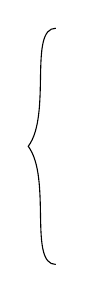
\begin{tikzpicture}\draw (0.35,0) .. controls (0,0) and (0.3,-1.1) .. (0,-1.5) .. controls (0.3,-1.9) and (0,-3) .. (0.35,-3);\end{tikzpicture}}
On écrit \unsure{d'abd.}
\[
i=u+pr,\quad j=v+ps\qquad0\leq u,v\leq p-1,\quad r,s\geq0
\]
et on montre que
\[
(*)\quad\begin{cases}
c_{ij}\not\equiv0\ (p)\quad\text{sss}\quad u+v\leq p-1\text{ et }c_{r,s}\not\equiv0\ (p)\\
c_{ij}\equiv c_{u,v}\,c_{r,s}\qquad(p)
\end{cases}
\]
en étudiant le développement, dans $\mathbb F_p[X,Y]$, de $(X+Y)^{i+j}$. \deleted{\unsure{On}} a
\[
i+j=p\underbrace{(r+s)}_t+\underbrace{u+v}_{\deleted{\unsure{v}}\inserted{w}}
\]
si $w\leq p-1$ on écrit
\[
\begin{aligned}
(X+Y)^{i+j}&=((X+Y)^p)^{\unsure{t}}(X+Y)^w=(X^p+Y^p)^{\unsure{t}}(X+Y)^w\\
&=\sum_{\substack{0\leq\alpha\leq w\\0\leq\beta\leq t}}\binom{w}{\alpha}\binom{t}{\beta}X^{\alpha+p\beta}Y^{(w-\alpha)+p(t-\beta)},
\end{aligned}
\]
où tous les monômes écrits dans la somme sont à exposants distincts. On a donc comme coeff. de $X^iY^j$ celui correspondant au terme $i=\alpha+p\beta$ i.e.
\[
\alpha=u,\quad\beta=r\qquad\text{i.e.}
\]
\[
c_{i,j}\equiv\binom{w}{u}\binom{t}{r}=c_{u,v}\,c_{r,s}\qquad(p)
\]
et il est immédiat que $c_{u,v}\not\equiv0\ (p)$, car $c_{u,v}=\dfrac{(u+v)!}{u!\,v!}$
\[
0\leq u,v,u+v\leq p-1.\qquad\text{Donc}\quad c_{ij}\not\equiv0\ (p)\Longleftrightarrow c_{r,s}\not\equiv0\ (p).
\]
Il reste à voir que si $w\geq p$, \deleted{soit $w=p+w'$} \inserted{alors} $c_{i,j}\equiv0\ (p)$
\[
\text{Soit }\unsure{w'|w}=p+w'\qquad0\leq w'\leq p-2,\quad\text{donc}\quad
\inserted{i+j=(r+s+1)p+w'=\underbrace{(t+1)}_{t'}p+w',}
\]
\[
(X+Y)^{i+j}=(X^p+Y^p)^{\unsure{t'}}(X+Y)^{w'}
=\sum_{\substack{0\leq\alpha\leq w'\\0\leq\beta\leq t'}}\binom{w'}{\alpha}\binom{t'}{\beta}X^{\alpha+\beta p}Y^{(w'-\alpha)+p(t'-\beta)}.
\]
\unsure{Trouver} un $X^iY^j$ correspondant à $\alpha=u,\beta=r$, il faudrait $u=\alpha\leq w'=u+v-p$ donc $v\geq p$, ce qui n'est pas, donc il n'y a pas de

\mspage{19}
\scanpage{21}

tels termes. Donc $c_{ij}\equiv0\ (p)$ dans ce cas, ce qui prouve (remplaçant $i,j$ par $u,v$) que $c_{u,v}\equiv0\ (p)$ donc encore $c_{ij}\equiv c_{u,v}c_{r,s}\ (p)$.

Le lemme 1 résulte du \unsure{corollaire} par une récurrence immédiate sur la longueur $e$ des développements $p$-adiques écrits de $u$ et de $v$.

\uline{Cor. 2} Soit $N$ un entier \inserted{$\geq0$} tel que $N+1\equiv0\ (p)$, posons
\figure{\begin{tikzpicture}\draw (0,0)--(0,-2.7);\end{tikzpicture}}
\[
N+1=(N'+1)p\quad\text{donc}\quad N=(N'+1)p-1=N'p+(p-1)
\]
(de sorte que à décalage de 1 près, les $N+1$ et $N'+1$ ont $=$ chiff. du développement $p$-adique, ainsi que $N$ et $N'$ (quand on fait abstraction du premier chiff. p.a. de $N$). Soit donc $\varepsilon\geq1$, on a
\[
\begin{aligned}
c_{N+1,p^\varepsilon-1}\deleted{\unsure{\not\equiv0\ (p)\Longleftrightarrow}}\inserted{\equiv}
c_{N'+1,p^{\varepsilon-1}-1}\deleted{\unsure{\not\equiv0\ (p)}}\deleted{\unsure{\ne0}}
\left\{\begin{array}{ll}
\equiv1\ (p)&\text{si }N'+1\equiv0\ (p^{\varepsilon-1})\\
\equiv0\ (p)&\text{si }N'+1\not\equiv0\ (p^{\varepsilon-1})
\end{array}\right.\\
c_{N,p^\varepsilon}\deleted{\unsure{\not\equiv0\ (p)\Longleftrightarrow}}\inserted{\equiv}
c_{N',p^{\varepsilon-1}}\deleted{\unsure{\not\equiv0}}\ (p)\deleted{\unsure{(p)}}
\left\{\begin{array}{l}\equiv v_{\varepsilon-1}+1\ (p)\quad(\text{si}\\
\deleted{\unsure{u_\alpha}}\quad N'=\sum v_\alpha p^\alpha)
\end{array}\right.
\end{aligned}
\]

\uline{Dém.} Le développement $p$-adique de $p^\varepsilon-1$ est
\[
p^\varepsilon-1=(p-1)+(p-1)p+\dots+(p-1)p^{\varepsilon-1}
\]
de m
\[
p^{\varepsilon-1}-1=(p-1)+\dots+(p-1)p^{\varepsilon-2}\quad\text{si }\varepsilon\geq2\quad(=0\text{ si }\varepsilon=1)
\]
Prenant
\[
\left.\begin{aligned}
N'+1&=u_0+u_1p+\dots+u_\nu p^\nu\\
N'&=v_0+v_1p+\dots+v_\nu p^\nu
\end{aligned}\right\}\quad(\nu\geq\varepsilon-1)
\]
d'où
\[
\begin{aligned}
N+1&=0+u_0p+u_1p^2+\dots+u_\nu p^{\nu+1}\\
N&=p-1+v_0p+v_1p^2+\dots+v_\nu p^{\nu+1}
\end{aligned}
\]
\uline{!} On trouve
\[
\begin{cases}
c_{N+1,p^\varepsilon-1}\equiv c_{u_0,p-1}\,c_{u_1,p-1}\dots c_{u_{\varepsilon-2},p-1}\quad(p)\quad(\equiv1\ \inserted{(p)}\text{ si }\varepsilon=1)\\
c_{N'+1,p^{\varepsilon-1}-1}\equiv c_{u_0,p-1}\,c_{u_1,p-1}\dots c_{u_{\varepsilon-2},p-1}\quad(p)\quad(\equiv1\ (p)\text{ si }\varepsilon=1)
\end{cases}
\]
\[
\begin{cases}
c_{N,p^\varepsilon}\equiv c_{v_{\varepsilon-1},1}\equiv v_{\varepsilon-1}+1\\
c_{N',p^{\varepsilon-1}}\equiv c_{v_{\varepsilon-1},1}\equiv v_{\varepsilon-1}+1
\end{cases}
\]

\margin{\uline{Rmq} \unsure{$\overline m$|même} si $E$ un $\mathbb F_p$-vectoriel, on \unsure{ne} peut conclure que $x_i=x_N$ $\forall i\in I$ (ex : \inserted{$p=2$,} $N=2$, $e=2$, donc on a $x_2,x_3,x_4,x_6$ on a $x_2=x_3=x_6$ mais \uline{pas} néc. $=x_4$)}
\deleted{\uline{\unsure{Prop}}}\inserted{\uline{Lemme 2}} Soit $\mathbb Z_p$ le localisé de $\mathbb Z$ en $p$, $E$ un $\mathbb Z_p$-module, $N\in\mathbb N$, $e\geq0$ tel que $p^e\geq N+1$, \deleted{\inserted{\unsure{(donc $e\geq1$)}}} $I$ l'ens. des entiers de la forme $N$ et $N+p^\varepsilon$, $0\leq\varepsilon\leq e$, $(x_i)_{i\in I}$ une famille d'éléments de $E$, tel qu'on ait
\figure{\begin{tikzpicture}\draw (0,0)--(0,-2.9);\end{tikzpicture}}
\[
\binom ji(x_j-x_i)=0\qquad i=N,N+1,\quad i<j\in I\quad(\text{donc }j=N+p^\varepsilon,\ 0\leq\varepsilon\leq e)
\]

\mspage{20}
\scanpage{22}

\deleted{\unsure{Lemme 3}} Alors on a $x_N=x_{N+1}$.

\uuline{Dém} Posons
\[
\begin{cases}
\deleted{\unsure{y_0=x_{N+1}-x_N}}\\
y_\varepsilon=x_{N+p^\varepsilon}-\unsure{x_N}\qquad0\leq\varepsilon\leq e.
\end{cases}
\]
d'où
\[
y_\varepsilon-y_0=x_{N+p^\varepsilon}-x_{N+1}
\]
\deleted{$\unsure{y'_\varepsilon=x_{N+p^\varepsilon}-x_{N+1}}$}

L'hypothèse s'écrit donc, en distinguant les cas $i=N$, $i=N+1$
\deleted{$\unsure{(N+1)y_0=0}$}\qquad\deleted{$\unsure{(i=N,\ j=N+p^\varepsilon)}$}
\[
(\unsure{S|\overline S})=S(N,e,(y_\varepsilon)_{0\leq\varepsilon\leq e})\quad
\begin{cases}
c_{N,p^\varepsilon}y_\varepsilon=0&0\leq\varepsilon\leq e\\
c_{N+1,p^\varepsilon-1}(y_\varepsilon-y_0)=0&0\leq\varepsilon\leq e\quad(\text{le cas }\varepsilon=0\text{ étant trivial})
\end{cases}
\]
La conclusion s'écrit $y_0=0$. En fait, nous allons déduire cette conclusion du système plus faible \inserted{(équivalent si $E$ est annulé par $p$, i.e. est un $\mathbb F_p$-vectoriel)}
\[
(\overline S')=\overline S(N,e,(y_\varepsilon)_{0\leq\varepsilon\leq e})\quad
\begin{cases}
y_\varepsilon=0\text{ si }c_{N,p^\varepsilon}\not\equiv0\ (p)&0\leq\varepsilon\leq e\\
y_\varepsilon-y_0=0\text{ si }c_{N+1,p^\varepsilon-1}\not\equiv0\ (p)&\unsure{1|0}\leq\varepsilon\leq e.
\end{cases}
\]

Pour prouver que ce système implique $y_0=0$, on récurre sur $N$. Comme la première équation pour $\varepsilon=0$ donne
\[
y_0=0\text{ si }N+1\not\equiv0\ (p)
\]
la conclusion est triviale pour $N=0$. \deleted{\unsure{Alors on}} On suppose donc $N>0$, \inserted{et prouvé pour les $N'<N$.} La conclusion est triviale si $N+1\not\equiv0\ (p)$.
Donc OPS
\[
N+1\equiv0\ (p)\quad\text{soit}\quad N+1=(N'+1)p
\]
où
\[
N'=\frac{N+1}{p}-1<N\qquad\left(\text{car }\frac{N+1}{p}<N+1\right).
\]
Alors le cor. précédent montre que le syst. $\overline S=\overline S(N,e,(y_\varepsilon)_{0\leq\varepsilon\leq e})$ \inserted{(compte tenu de $N+1\equiv0\ (p)$ qui nous permet d'oublier la première équation pour $\varepsilon=0$)} équivaut au système (où $e'=e-1$, $y'_\varepsilon=y_{\varepsilon+1}$ pour $0\leq\varepsilon\leq e'=e-1$)
\[
\deleted{\overline S'=\overline S'(N',e',(y'_\varepsilon)_{\unsure{1\leq\varepsilon}})}\quad
\begin{cases}
y'_\varepsilon=0\text{ si }c_{N',p^\varepsilon}\not\equiv0\ (p)&0\leq\varepsilon\unsure{=|\leq}e'\\
y'_\varepsilon-y_0=0\text{ si }c_{N'+1,p^\varepsilon-1}\not\equiv0\ (p)&\unsure{0|1}\leq\varepsilon\leq e'
\end{cases}
\]
Pour $\varepsilon=0$ cette dernière équation donne \deleted{$\unsure{x}$}
\[
y'_0=y_0
\]
donc on peut se borner à $1\leq\varepsilon\leq e'$ (et se rappeler $y'_0=y_0$).

\mspage{21}
\scanpage{23}

Mais alors ce système n'est autre que
\[
\overline S'=\overline S'(N',e',(y'_\varepsilon)_{0\leq\varepsilon\leq e'}).
\]
Notons que $p^e\geq N+1=(N'+1)p$ implique $p^{e-1}\geq N'+1$ i.e. $p^{e'}\geq N'+1$. Donc on est dans les $=$s conditions que précédemment, avec cette fois-ci $N'<N$. Par hyp. de récurrence on a donc $y'_0=0$, donc $y_0=0$, cqfd. Ouf !

\uline{Théorème 1} Soient $E$ un \unsure{groupe} abélien, $N\in\mathbb N$, $(x_i)_{i\in\mathbb N}$ une famille d'éléments de $E$, telle qu'on ait
\figure{\begin{tikzpicture}\draw (0,0)--(0,-1.4);\end{tikzpicture}}
\[
\binom ji(x_j-x_i)=0\qquad\text{pour }j>i\geq N
\]
Alors on a $x_i=x_N$ $\forall i\geq N$.

\uline{Dém} Quitte à localiser en tous les nbs premiers $p$, OPS $E$ un module sur \inserted{un} $\mathbb Z_p$. Il suffit de prouver $x_{N+1}=x_N$ (car par récurrence on tire de m $x_{N+1}=x_{N+2}$ etc). Choisissons $e$ \inserted{$\in\mathbb N$} tel que $p^e\geq N+1$, n'utilisons que les $x_i$ pour $i$ de la forme $N$ ou $N+p^\varepsilon$, $0\leq\varepsilon\leq e$. Le lemme 2 nous montre que $x_{N+1}=x_N$, cqfd.

\uline{Cor 1} Soient $k$ un anneau commutatif, $S=k\{T\}$ l'alg. des polynômes à puiss. div., \deleted{M un $k$-module, $\unsure{S,S^{+(N)}}$} \deleted{\unsure{M}}\inserted{$S^{+(N)}$} l'idéal à p.div. \deleted{engendré par $\unsure{T^{(N)}}$} défini par
\[
S^{+(N)}=\sum_{i\geq N}k.T^{(i)}.
\]
et considérons, pour $\forall$ $k$-module $M$, le $S$-module gradué
\[
\deleted{\unsure{a}}\quad\omega_N(M)=M\otimes_S S^{+(N)}=\sum_{i\geq N}M.T^{(i)}
\]
Alors :

\mspage{22}
\scanpage{24}
\figure{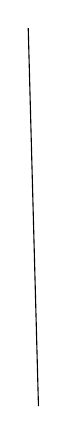
\begin{tikzpicture}\draw (0,0) -- (0.13,-4.8);\end{tikzpicture}}

a) Le foncteur $\omega_N$ (de la catégorie des $k$-modules vers celle des $S$-modules gradués) est pleinement fidèle.

b) \inserted{$\forall M$,} l'application
\diagram{\begin{tikzcd}
M \arrow[r,"\varphi"] & \displaystyle\prod_{i\geq0}\omega_N(M)_i=\prod_{i\geq N}M.T^{(i)}
\end{tikzcd}}
donnée par
\[
\varphi(x)=(x.T^{(i)})_{i\geq N}
\]
induit une bijection de $M$ avec le sous-ens. de $\prod_{i\geq N}\deleted{\unsure{M}}\omega_N(M)_i$ formé des systèmes $(x_i)_{i\geq N}$ satisfaisant la condition
\[
(*)\qquad T^{(j)}x_i=c_{ij}x_{i+j}\qquad\forall i\geq N,\ j\geq1.
\]

\uline{Dém}

b) $x_i=xT^{(i)}$, on a $T^{(j)}x_i=xT^{(i)}T^{(j)}=c_{ij}xT^{(i+j)}=c_{ij}x_{i+j}$, donc $\varphi(x)$ se trouve dans le sous-gr. indiqué.

L'injectivité de $\varphi$ est claire. Bijectivité? Posons $x_i=\unsure{\xi_i|\zeta_i}T^{(i)}$, $\unsure{\xi_i|\zeta_i}\in M$. La condition $(*)$ s'écrit
\[
\begin{array}{ccc}
\xi_iT^{(i)}T^{(j)}&=&c_{ij}\xi_{i+j}T^{(i+j)}\\
\text{''}&&\\
c_{ij}\xi_iT^{(i+j)}&&
\end{array}
\]
i.e.
\[
c_{ij}(\xi_{i+j}-\xi_i)=0\qquad\text{pour }i\geq N,\ j\geq1,
\]
et il résulte du th. que les $\xi_i$ sont tous \uline{égaux} à un $=\xi\in M$, cqfd.

a) Soient $M,M'$ sur $k$. Alors $\operatorname{Hom}(\omega_N(M),\omega_N(M'))$ s'identifie à l'ens des systèmes de $k$-lin $(i\geq N)$
\diagram{\begin{tikzcd}
u_i:\ M \arrow[r,dash] \arrow[d,phantom,"\unsure{\wr|\simeq}" description] & M' \arrow[d,phantom,"\unsure{\wr|\simeq}" description]\\
M.T^{(i)} \arrow[d,phantom,"\text{''}" description] & M'.T^{(i)} \arrow[d,phantom,"\text{''}" description]\\
\omega_N(M)_i & \omega_N(M')_i
\end{tikzcd}}
\mspage{23}
\scanpage{25}
tels que $\forall j\geq1$, on ait comm. dans
\diagram{\begin{tikzcd}
M.T^{(i)} \arrow[r,".T^{(j)}"] \arrow[d,"u_i\otimes T^{(i)}"'] & MT^{(i+j)} \arrow[d,"u_{i+j}\otimes T^{(i+j)}"]\\
M'.T^{(i)} \arrow[r,".T^{(j)}"] & M'.T^{(i+j)}
\end{tikzcd}}
i.e. tels qu'on ait
\[
c_{ij}(u_{i+j}-u_i)=0\qquad\text{si }i\geq N,\ j\geq1,
\]
et le th. nous permet de conclure que tous les $u_i$ sont égaux, d'où la conclusion
\diagram{\begin{tikzcd}
\operatorname{Hom}_k(M,M') \arrow[r,"\sim"] & \operatorname{Hom}_{\unsure{S\text{-mod gr.d}|S\text{-mod gr.}}}(\omega_N(M),\omega_N(M'))
\end{tikzcd}}

\uline{Rmq 1} Le foncteur $\omega_N$ admet un adjoint à droite $\pi_N$
\[
\operatorname{Hom}_{\unsure{S\text{-mod gr.d}|S\text{-mod gr.}}}(\omega_N(M),\unsure{\mathcal M})\simeq\operatorname{Hom}_k(M,\pi_N(\mathcal M))
\]
en posant
\[
\begin{array}{l}
\pi_N(\mathcal M)\subset\displaystyle\prod_{i\geq N}\mathcal M_i\\
\qquad\text{''}\\
\displaystyle\left\{(x_i)_{i\geq N}\ \middle|\ x_iT^{(j)}=c_{ij}x_{i+j}\quad\forall i\geq N,\ j\geq1\right\}
\end{array}
\]
En considération de ceci, \deleted{il existe} les parties a) et b) du corollaire 1 sont équivalentes, b) signifie que l'hom. can. d'adjonction
\diagram{\begin{tikzcd}
M \arrow[r] & \pi_N(\omega_N(M))
\end{tikzcd}}
est \deleted{\unsure{tjs|tjrs}} un isomorphisme.

\uline{Rmq 2} Considérons $\omega_0(M)=M\otimes_k S=M\otimes_k k\{T\}$, alors $\omega_N(M)=S^{+(N)}.\omega_0(M)$. \deleted{Donc $\unsure{\omega_N}$ \unsure{en un sens}, $\unsure{\omega_0\to}$} \inserted{On peut aussi écrire, si $N\geq N'\geq0$}
\[
\omega_N(M)\simeq\deleted{\unsure{\prod}}\sum_{i\geq N}\omega_{N'}(M)_i\overset{\mathrm{def}}=\underset{\text{(``troncature'')}}{\tau_{\geq N}}(\omega_{N'}(M)).
\]
Donc en
\mspage{24}
\scanpage{26}
un sens les foncteurs ``ombres'' $\omega_N$ sont d'autant plus grossiers que $N$ est plus grand. Néanmoins ils sont tous pleinement fidèles (\uline{NB} les foncteurs $\tau_N$ ne sont pas pl. fidèles bien sûr, pas $=$ sur la sous-catégorie des ``ombres virtuelles d'ordre $N-1$'', i.e. des modules gradués dont les composantes sont nulles en degrés $\leq N-1$.

Soit $\operatorname{Omb}(k)$ la catégorie des ``ombres virtuelles'' des $k$-modules, i.e. des $S=k\{T\}$-modules gradués [à degrés $\geq0$?]. Soit, $\forall N\geq0$, $\operatorname{Omb}_{\unsure{N\text{-n}}}(k)$ la sous-catégorie pleine des modules $N$-négligeables, i.e. tels que $\mathcal M_i=0$ si $i\geq N$.
C'est une sous-catégorie épaisse, la catégorie quotient est can. équivalente \deleted{à celle} \inserted{\unsure{la s-cat. pleine de (Omb) formée}} des ``\inserted{$N$-}ombres virtuelles'', i.e. des $\unsure{S|k}$-modules gradués tels que $\mathcal M_i=0$ si $i<N$.
Le foncteur passage au quotient s'identifie alors au foncteur ``troncature'' $\tau_N$. On note que
\diagram{\begin{tikzcd}
\tau_N(\mathcal M) \arrow[r,hook] & \mathcal M
\end{tikzcd}}
(inclusion fonctorielle) \inserted{correspond au fait que} le foncteur \deleted{$\unsure{\tau_N}$} pass. au quotient admet un adjoint à droite (pl. fid. comme de juste)
\[
\operatorname{Hom}_{\operatorname{Omb}}(\mathcal N,\tau_N(\mathcal M))\simeq
\operatorname{Hom}_{\substack{N\text{-Omb}\\\text{ou Omb}}}(\tau_N(\unsure{\mathcal M|\mathcal N}),\tau_N(\mathcal M)).
\]

Appelons ``négligeable'' une ombre $\mathcal M$ qui est $\varinjlim$ \inserted{filtr.} d'ombres $N$-négligeables (pour $N$ variable), i.e. telle que \inserted{$\forall i\in\mathbb Z$,} $\forall x\in\mathcal M_i$, $\exists N\unsure{(\in\mathbb N)}$ tel que $T^{(\alpha)}.x=0$ pour $\alpha\geq N$ i.e. $S^{+(N)}.x=0$. C'est encore une sous-catégorie épaisse, et le localisé est
\mspage{25}
\scanpage{27}
$S=k\{T\}$ (polynômes à p.d.) anneau gradué à degrés $\geq0$,
$M$ un $k$-module, $N\geq0$, d'où $M\otimes_kS$ et par suite
\diagram{\begin{tikzcd}
M\otimes_kS \arrow[r] & \unsure{\varphi_N|\rho_N}\tau_N(M\otimes_kS)
\end{tikzcd}}
\uline{Thm} L'hom précédent est un isom en degrés $\geq0$, i.e. on a
\diagram{\begin{tikzcd}
(\alpha)\qquad M\otimes_kS \arrow[r,"\sim"] & \unsure{\varphi_{0N}|\rho_{0N}}\tau_N(M\otimes_kS)
\end{tikzcd}}
Enoncé équivalent:
\[
M\otimes_kS\in\operatorname{Im\,ess}\varphi_{0N}\qquad(\forall N\geq0)
\]
ou encore
\[
M\otimes_kS\in\operatorname{Im\,ess}\varphi_{0,\infty}
\]

\uline{NB} En degrés $\geq N$, c'est clair que $\alpha$ est un isom, il suffit donc de regarder les degrés $0\leq i<N$. Le cas $i=0$ a été traité déjà par une démonstration spéciale (\unsure{on la retrouvera} dans \unsure{la dém. qui va suivre}).

Reformulation du \uline{Thm}

Si $0\leq i\leq N$, \unsure{on a}
\diagram{\begin{tikzcd}
\left(\begin{array}{c}\xi T^{(i)}\\\uparrow\\\xi\end{array}\right) & (M\otimes_k\unsure{S})_i \arrow[r,"\sim"] & \operatorname{Hom}^{i}(\tau_{N-i}(S),M\otimes_kS)\\
& M \arrow[u,phantom,"\wr" description] &
\end{tikzcd}}
(seul le cas $0\leq i<N$ doit être établi)

\uline{Cor}
\[
\operatorname{Ext}^n(\tau_{N-i}(S)[-i],M\otimes_kS)=0\quad\text{si }n>0
\]
$\forall i\geq0$ (seul le cas $i<N$ est non trivial \deleted{$\unsure{0\leq i}$})

Ce théorème équivaut à l'énoncé suivant, où $k$ ne figure plus

\uline{Th} Soient $0\leq i\leq N$ deux entiers, $M$ un $\mathbf Z$-module, $(\xi_k)_{k\geq N}$ une famille d'éléments de $M$, telle que l'on ait
\figure{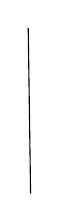
\begin{tikzpicture}\draw (0,0) -- (0.03,-2.1);\end{tikzpicture}}
\[
(1)\qquad c_{\ell,k}\xi_k=c_{\ell,k-i}\xi_{k+\ell}\qquad\text{pour }k\geq N,\ \ell\geq0
\]
\mspage{26}
\scanpage{28}
Alors il existe un unique $\xi\in M$ tel que l'on ait
\[
(2)\qquad\xi_k=c_{\unsure{i},k-i}\xi\quad\left(=\binom{k}{i}\xi\right)\quad\text{pour }\forall k\geq N
\]
(\uline{NB} $c_{k,\ell}$ désigne le coefficient binômial $\dfrac{(k+\ell)!}{k!\ell!}$)

\uline{Dém} \textcircled{1} Réduction au cas où $\exists p$ nb premier, tel que $\unsure{n}\operatorname{id}_M$ bijectif $\forall n\in\mathbf Z$ tel que $(n,p)=1$, i.e. $M$ un $\mathbf Z_p$-module ($\mathbf Z_p\overset{\mathrm{def}}=\mathbf Z_{(p\mathbf Z)}$).
Supposons que ce soit prouvé dans ce cas, et qu'on sache qu'il existe alors $k=k(p)$ tel que $\deleted{\unsure{\xi}}c_{i,k-i}\not\equiv0\ (p)$ (i.e. $c_{k,k-i}\in\mathbf Z_p^*$). Prouvons le th. en général. Les $c_{k,k-i}$ $(k\geq N)$ ne sont pas divisibles par un $=$ nb premier, donc sont premiers dans leur ensemble, donc $\exists k_1\ldots k_r\geq N$ et des entiers $m_1,\ldots m_r\in\mathbf Z$ tels que
\[
\sum_{\alpha=1}^{r}m_\alpha c_{k_\alpha,k_\alpha-i}=1.
\]
Donc les relations (2) impliquent, en multipliant par les $m_\alpha$ et sommant
\[
\xi=\sum_1^r m_\alpha\xi_{k_\alpha}
\]
d'où l'unicité de $\xi$. Prouvons qu'avec ce choix de $\xi$, on a bien (2) i.e.
\[
\xi_k=c_{k,k-i}\sum_1^r m_\alpha\xi_{k_\alpha}
\]
Pour prouver que cette relation est vraie, \deleted{\unsure{Alors}} il suffit de prouver qu'elle est vraie dans chaque $M_p=M\otimes_{\mathbf Z}\mathbf Z_p$ $(p\in\mathbf P)$. Mais c'est une conséquence immédiate du fait que le th. est vrai pour $M_p$.
\mspage{27}
\scanpage{29}
\textcircled{2} Cas où $M$ est un $\mathbf Z_p$-module

Notons d'abord qu'il existe des $k$ arbitrairement grands tels que $c_{i,k-i}\in\mathbf Z_p^*$ i.e. $c_{i,k-i}\not\equiv0\ (p)$. Posons $k-i=j$, il suffit de prendre $j=p^\varepsilon$, avec $\varepsilon$ tel que $p^\varepsilon>i$, donc $k=i+p^\varepsilon$. Cela montre l'unicité de $\xi$, car si $k_0$ est tel que $c_{i,k_0-i}\in\mathbf Z_p^*$, on aura
\[
\deleted{\unsure{(\alpha)|(2)}}\qquad\xi=c_{i,k_0-i}^{-1}\xi_{k_0}
\]
Considérons alors le système des
\[
\deleted{\unsure{(\beta)|(3)}}\qquad\xi'_k=c_{i,k-i}\xi,
\]
on voit de suite \deleted{\unsure{ainsi que}} que \deleted{\unsure{on}} $(\xi'_k)_{k\geq N}$ satisfait les conditions (1), (où on substitue $\xi'_k$ à $\xi_k$), et $\xi'_{k_0}=\xi_{k_0}$, donc posons
\[
\eta_k=\xi'_k-\xi_k,
\]
\deleted{les} $(\eta_k)_{k\geq N}$ satisfait encore (1), et de plus $\eta_{k_0}=0$. Il suffit de prouver alors $\eta_k=0$, \deleted{\unsure{d'où}} $\forall k\geq N$. Donc on est ramené au

\uline{Corollaire} Si $(\xi_k)_{k\geq N}$ \deleted{est} satisfait (1), et \inserted{si} de plus \deleted{$\unsure{(1')}$} \unsure{on a donné} un $k_0\geq N$ tel que
\figure{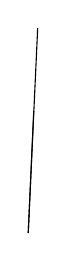
\begin{tikzpicture}\draw (0,0) -- (-0.12,-2.6);\draw (-0.05,-1.05) -- (-0.12,-2.6);\end{tikzpicture}}
\[
(1')\qquad\xi_{k_0}=0
\]
\[
(3)\qquad c_{i,k_0-i}\not\equiv0\ (p)
\]
alors $\xi_k=0\qquad\forall k>N$.
\mspage{28}
\scanpage{30}
\uline{Dém} En deux étapes

\uline{LEMME 1} $\xi_k=0$ si \inserted{$k\geq N$ tel que} $c_{i,k-i}\not\equiv0\ (p)$

\uline{Lemme} 1.1. Soient \deleted{$\unsure{k,k'}$} $k'\geq k\geq N$ tels que, posant $j=k-i$, $j'=k'-i\unsure{\deleted{j}|^\ast}$, on ait
\[
(4)\qquad c_{i,j}\not\equiv0\ (p)\quad\text{et}\quad c_{i,j'}\not\equiv0\ (p)
\]
Alors on a l'équivalence
\[
(5)\qquad c_{j'-j,j}\not\equiv0\ (p)\quad\Longleftrightarrow\quad c_{j'-j,j+\unsure{i|j}}\not\equiv0\ (p)
\]
et si les conditions équivalentes (5) sont satisfaites, on a l'équivalence
\[
(6)\qquad\xi_k=0\quad\Longleftrightarrow\quad\xi_{k'}=0.
\]

\uline{Dém de} 1.1. Calculons dans $\mathbf Q$
\[
\text{(a)}\quad c_{j'-j,j+i}/c_{j'-j,j}=\frac{(j'+i)!}{\deleted{(j'-j)!}(j+i)!}:\frac{(j'\deleted{+\unsure{i|j}})!}{\deleted{(j'-j)!}j!}
\]
\margin{$\unsure{\alpha\ //}$}
\[
\text{(b)}\quad c_{i,j'}/c_{ij}=\frac{(i+j')!}{\deleted{i!}j'!}:\frac{(i+j)!}{\deleted{i!}j!}
\]
\deleted{\[
\text{(b)}\quad c_{ij'}/c_{ij}=\frac{(i+j')!}{i!j'!}:\frac{(i+j)!}{i!j!}
\]
le quotient de (a) et (b) \unsure{est}, grâce à (4)
\[
(i+j)!\sim i!j!\qquad(i+j')!\unsure{\simeq|\sim}i!j'!
\]
donc le premier \unsure{mb.} de (a) est égal à
\[
\frac{i!j'!}{i!j!}:\frac{(j'+i-j)!}{\unsure{i!}}=
\]}
\margin{\deleted{Or dans $\mathbf Z_p$ pour ce rel. de divisibilité, on}}
\figure{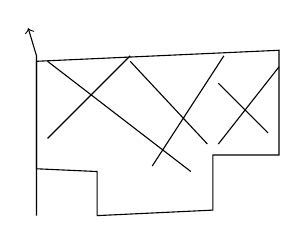
\begin{tikzpicture}[scale=.7]
\draw[->] (0,0)--(0,2.9)--(-.15,3.4);
\draw (0,2.8)--(4.4,3)--(4.4,1.1)--(3.2,1.1)--(3.2,.1)--(1.1,0)--(1.1,.8)--(0,.85)--cycle;
\draw (.2,2.8)--(2.8,.8) (.2,1.4)--(1.7,2.9) (1.7,2.8)--(3.1,1.3) (2.1,.9)--(3.4,2.9) (3.3,2.4)--(4.2,1.5) (3.3,1.3)--(4.4,2.7);
\end{tikzpicture}}
Donc les deux quantités (a) et (b) sont \unsure{égaux|égales}, et comme (b) est un quotient de deux unités \deleted{p-adiques} \inserted{de $\mathbf Z_p$}, on voit que $c_{j'-j,j+i}$ et $c_{j'-j,j}$ sont \unsure{équivalents|équivalent} pour la divisibilité, donc l'un est une \unsure{unité|unit} ssi l'autre l'est. Quand il en est ainsi, la
\mspage{29}
\scanpage{31}
relation (1) avec $\ell=k'-k=j'-j$ donne
\[
c_{j'-j,j+i}\xi_k=c_{j'-j,j}\xi_{k'}\deleted{\unsure{k}}
\]
et comme les coeff \unsure{sont} des unités de $\mathbf Z_p$, on en conclut que $\xi_k=0\quad\Longleftrightarrow\quad\xi_{k'}=0$, cqfd.

\uline{Dém du lemme 1} Considérons le développement $p$-adique de $i$
\[
i=i_0+i_1p+\cdots+i_rp^r\qquad0\leq i_\alpha\leq p-1\quad(0\leq\alpha\leq r)
\]
où on prendra $r$ arbitrairement grand (car on suppose \deleted{\unsure{avec}} \uline{pas} que $i_r\ne0$!). Considérons de $=$ \deleted{\unsure{le}} développement de $j=k-i$
\[
j=j_0+j_1p+\cdots+j_rp^r\qquad0\leq j_\alpha\leq p-1\quad(0\leq\alpha\leq r)
\]
L'hyp. $c_{i,j}\not\equiv0\ (p)$ signifie que
\[
i_\alpha+j_\alpha\leq p-1\qquad\forall\ 0\leq\alpha\leq r
\]
Soit \deleted{$\unsure{\varepsilon_\alpha}$}
\[
\delta_\alpha=(p-1)-(i_\alpha+j_\alpha)\qquad0\leq\delta_\alpha\leq p-1
\]
i.e.
\[
j'_\alpha\overset{\mathrm{def}}=j_\alpha+\delta_\alpha=(p-1)-i_\alpha
\]
donc
\[
0\leq j'_\alpha\leq p-1
\]
et considérons
\[
j'=\sum_0^r j'_\alpha p^\alpha
\]
donc $j'\geq j\ (\unsure{\geq|>}N)$ et
\[
j'-j=\delta\overset{\mathrm{def}}=\sum_0^r\delta_\alpha p^\alpha
\]
On a alors \inserted{(en plus de $c_{i,j}\not\equiv0$!)}
\[
c_{i,j'}\not\equiv0\ (p)\qquad\text{car }i_\alpha+j'_\alpha\ (=p-1)\leq p-1\quad\forall\alpha
\]
\[
c_{j'-j,j}\unsure{=|\not\equiv}c_{\delta,j}\not\equiv0\ (p)\quad\text{car }\delta_\alpha+j_\alpha=j'_\alpha\leq p-1
\]
\margin{\uline{Présentation plus simple} Soit $r\geq0$ tel que $p^r>\deleted{\unsure{i}}i+j$.
Soit \deleted{$\delta=\unsure{p^r-1}$} $\delta=p^r-1-(i+j)$ d'où $i+j+\delta=p^r-1$.
$\unsure{(i+j+\delta)=}$
Alors on a
\[
\begin{cases}
c_{i,j+\delta}\not\equiv0\ (p)\\
c_{(i+j),\delta}\not\equiv0\ (p)
\end{cases}
\]
(en plus de $c_{ij}\not\equiv0\ (p)$) donc
\[
\xi_k=0\quad\Longleftrightarrow\quad\xi_{k'}=0,\quad\text{\unsure{i.e.|où} }k'=j'+i=j+\delta+i=p^r-1
\]}
\figure{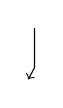
\begin{tikzpicture}\draw[->] (0,0)--(0,-.5)--(-.08,-.65);\end{tikzpicture}}
\mspage{30}
\scanpage{32}
donc en vertu de (1.1) on a
\[
\xi_k=0\quad\Longleftrightarrow\quad\xi_{k'}=0
\]
où $k'=i+j'=\sum_0^r(p-1)p^\alpha=p^{r+1}-1$,
donc on trouve que
\[
\xi_k=0\quad\Longleftrightarrow\quad\xi_{p^{r+1}-1}=0
\]
Pour la $=$ raison, on trouve, si $\widetilde k\deleted{\unsure{k_0}}\inserted{=i+\widetilde j}$ satisfait les $=$ conditions que $k$, savoir $c_{i,\unsure{k'|\widetilde k}-i}=0$
\[
\xi_{\widetilde k}=0\quad\Longleftrightarrow\quad\xi_{p^{r+1}-1}=0
\]
où on choisit $r$ tel que $p^{r+1}\geq\deleted{\unsure{k}}j,\widetilde j\ \unsure{(\geq i)}$.
En comparant, on trouve
\[
\xi_k=0\quad\Longleftrightarrow\quad\xi_{\widetilde k}=0
\]
i.e. si \uline{un} $\xi_k$ avec $k\geq N$, $c_{k,k-i}\not\equiv0\ (p)$ est nul, tous le sont, cqfd.

\uline{Fin de la démonstration}. Il \deleted{suffit de} \inserted{faut prouver} $\xi_k=0\quad\forall k\geq N$. On a
\[
c_{\ell,k}\xi_k=c_{\ell,k-i}\xi_{k+\ell}\qquad\forall\ell\geq0
\]
et il suffit de prouver qu'il existe $\ell\geq0$ tel que $c_{\ell,k}\not\equiv0\ (p)$, et de plus $\xi_{k+\ell}=0$, ce qui est le cas \deleted{si} en vertu de 1.1. si $c_{i,(k+\ell)-i}\not\equiv0\ (p)$. Posons encore $k-i=j$ i.e. $k=i+j$, on veut
\mspage{31}
\scanpage{33}
donc $c_{\ell,i+j}$ et $c_{\ell+j,i}\not\equiv0\ (p)$. C'est le contenu du

\uline{Lemme 2} Soient $i,j\geq0$. Alors il existe $\ell\geq0$ tel que $\deleted{\unsure{c_{ij\ell}}}c_{i+j,\ell}$ et $c_{i,j+\ell}$ soient $\not\equiv0\ (p)$.
\figure{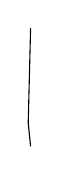
\begin{tikzpicture}\draw (0,0)--(-.03,-1.2)--(0,-1.5);\end{tikzpicture}}

\deleted{\uline{Dém} Considérons les développements $p$-adiques de $i$ et $j$
\[
i=i_0+i_1p+\cdots+i_rp^r
\]
\[
j=j_0+j_1p+\cdots+j_rp^r
\]
alors le développement $p$-adique de $\inserted{\sigma=}i+j$ est
\inserted{$\deleted{\unsure{i+}}j=\sigma=\sigma_0+\sigma_1p+\cdots+\sigma_{r+1}p^{r+1}$}
donné par le procédé \unsure{vraiment|couramment} bien connu, où on détermine par récurrence les couples d'entiers $\sigma_\alpha,\deleted{\unsure{\rho_\alpha}}$ $(0\leq\alpha\leq r+1)$ \inserted{et $\rho_\alpha$ $(-1\leq\alpha\leq r)$} --- les $\rho_\alpha$ sont les ``retenues'', égales à $0$ ou $1$ --- en posant \deleted{$\unsure{\rho_0=0}$}
\[
\textcircled{a}\quad\rho_{-1}=0,
\]
puis par récurrence par
\inserted{$0\leq\alpha\leq r$}
\[
\textcircled{b}\quad i_\alpha+j_\alpha+\rho_{\alpha-1}=\sigma_\alpha+p\rho_\alpha\qquad0\leq\sigma_\alpha,\rho_\alpha\leq p-1
\]
\margin{celà détermine $\sigma_\alpha$ et $\rho_\alpha$}
enfin
\[
\textcircled{c}\quad\sigma_{\unsure{\alpha|r}+1}=\rho_{\unsure{r}}
\]
Posons
\[
\ell_\alpha=(p-1)-\sigma_\alpha\qquad0\leq\alpha\leq r+1
\]
\[
\ell=\sum_0^{r+1}\ell_\alpha p^\alpha
\]
d'où $\sigma+\ell=\sum_0^{r+1}(p-1)p^\alpha=p^{r+2}-1$ i.e. $\ell=p^{r+2}-1-\sigma$.
On a alors, grâce à (b)
\[
\textcircled{a'}\quad\rho_{-1}=0
\]
\[
\textcircled{b'}\quad\text{Si }0\leq\alpha\leq r,\qquad(i_\alpha+j_\alpha+\ell_\alpha)+\rho_{\alpha-1}=(p-1)+p\rho_\alpha
\]
\margin{(où $\rho_{\alpha-1}$ et $\rho_\alpha$ sont $0\leq\ \leq p-1$)}
\[
\textcircled{b'}\mathrm{bis}\quad\deleted{\unsure{\alpha}}\underset{\substack{\text{''}\\0}}{i_{r+1}}+\underset{\substack{\text{''}\\0}}{j_{r+1}}+\ell_{r+1}+\rho_r=(p-1)+p.0
\]
\deleted{$\textcircled{c'}\quad\unsure{i_{r+1}+j_{r+1}}$}
Ce qui montre que \deleted{\unsure{inject.}} l'addition de}
\mspage{32}
\scanpage{34}
\deleted{entiers $i,j,\ell$, \unsure{donnés} par leurs développements $p$-adiques}

Soit $r\geq0$ tel que $p^r>i+j$, soit \deleted{$\unsure{\ell}$}
\[
\ell=p^r-1-(i+j)
\]
\deleted{Je dis que}
de sorte que l'on a
\[
i+j+\ell=p^r-1=\sum_{\alpha=0}^{r-1}(p-1)p^\alpha
\]
\inserted{$(i+j)+\ell=i+(j+\ell)$}
On sait alors, par le critère habituel, que l'on a $c_{i+j,\ell}\not\equiv0\ (p)$, et pour la $=$ raison on a $c_{i,j+\ell}\not\equiv0\ (p)$

cqfd

\uline{NB} Le lemme commun qui a servi dans les lemmes 1 et 2 est le suivant:
Si $\mu,\nu\geq0$ sont tels que
\[
\mu+\nu=p^r-1\qquad(r\geq0\text{ convenable})
\]
alors
\[
c_{\mu,\nu}\not\equiv0\ (p)
\]
\deleted{(plus précisément, $\unsure{c_{\mu,\nu}}$}
\margin{\unsure{5|S}}
\mspage{33}
\scanpage{35}
\[
\boxed{\unsure{\nu_p|v_p}(n!)=\frac{n-\mathrm{chif}_p n}{p-1}}
\]
\[
\deleted{\unsure{\nu_p(n!)|v_p(n!)}}\quad \unsure{\nu_p|v_p}\left(\frac{p^n}{n!}\right)=n-\frac{n-\mathrm{chif}_p n}{p-1}=\frac{\mathrm{chif}_p n+n(p-2)}{p-1}
\]
\figure{\begin{tikzpicture}\draw (0,.65)--(0,0)--(3.8,.05);\end{tikzpicture}}
\[
n=\sum_{\alpha\geq0}n_\alpha p^\alpha\qquad n-\mathrm{chif}_p n=\sum n_\alpha(p^\alpha-1)
\]
\[
\mathrm{chif}_p n=\sum n_\alpha\qquad\frac{n-\mathrm{chif}_p n}{p-1}=\sum_\alpha n_\alpha(1+\cdots+p^{\alpha-1})
\]
\[
\unsure{\nu_p|v_p}((n+1)!)=
\]
\figure{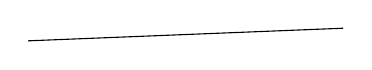
\begin{tikzpicture}\draw (0,0)--(4,.16);\end{tikzpicture}}
\[
\begin{aligned}
\unsure{\nu_p|v_p}\left(\frac{p^{r+1}!}{(p^r!)^p p!}\right)
&=\underbrace{\unsure{\nu_p|v_p}(p^{r+1}!)}_{\frac{p^{r+1}-1}{p-1}}
-p\underbrace{\unsure{\nu_p|v_p}(p^r!)}_{\frac{p^r-1}{p-1}}
-\underbrace{\unsure{\nu_p|v_p}(p!)}_{1}\\
&=0
\end{aligned}
\]
\mspage{34}
\scanpage{36}
aux homomorphismes
\diagram{\begin{tikzcd}
T \arrow[r] & A^{\unsure{\natural|\sharp}} \arrow[r] & A
\end{tikzcd}},
\margin{$\unsure{=}$}
nous montre alors aussitôt que $\uline{F}(A^\natural)$ et $\uline{F}(T)$ s'identifient respectivement à
\[
(13.4.10)\qquad\uline{F}(A^\natural)\simeq\uline{F}^{f}\overset{\mathrm{dfn}}=\uline{F}\cap\mathcal E^{f},\quad\uline{F}(T)=\uline{F}^{t}=\uline{F}\cap\mathcal E^{t}=0,
\]
le $=0$ provenant du fait immédiat que pour un tore $T$, on a $\uline{F}(T)=0$,
la suite exacte du type (13.4.3) devenant ici
\diagram{\begin{tikzcd}
0 \arrow[r] & 0 \arrow[r] & \mathcal E(T) \arrow[r] & \uline{\operatorname{Lie}}'(T) \arrow[r] & 0
\end{tikzcd}}.
On voit donc en même temps que l'homomorphisme composé
\diagram{\begin{tikzcd}
\mathcal E^{t} \arrow[r] & \mathcal E \arrow[r] & \uline{E}
\end{tikzcd}}
\margin{$\unsure{-}$}
induit un isomorphisme

\margin{495}
\figure{\begin{tikzpicture}\draw (0,0)--(.36,-.03);\end{tikzpicture}}
\margin{$\unsure{0=}$}
\fbox{495}
\mspage{35}
\scanpage{37}
\[
\begin{aligned}
\operatorname{Hom}^d(M^*,\varphi_NN^*)&=\operatorname{Hom}(M^*[-d],\varphi_NN^*)\\
&\simeq\operatorname{Hom}(\tau_N(M^*[-d]),N^*)\\
&\simeq\operatorname{Hom}((\tau_{N-d}M^*)[-d],N^*)\\
&\simeq\operatorname{Hom}^d(\tau_{N-d}M^*,N^*)
\end{aligned}
\]
\margin{$N^*\in\operatorname{Ob}\mathcal M_N$}
\[
\boxed{\operatorname{Hom}^d(M^*,\varphi_NN^*)\simeq\operatorname{Hom}^d(\tau_{N-d}M^*,N^*)}
\]
\uline{Supposons}
\[
M^*\in\unsure{\mathcal M_{-d}^{*}|\mathcal M_{-d}}\ [\text{i.e. }M^j=0\text{ si }j<-d],
\]
\[
N^*=\tau_N\mathbf N\otimes_kS_k=\tau_N\mathbf N_{S_k}\quad(\mathbf N\text{ un }k\text{-module})\qquad N\geq0
\]
Alors
\[
\begin{aligned}
\operatorname{Hom}^d(M^*,\varphi_N\tau_N\mathbf N^*_{S_k})
&=\operatorname{Hom}^d\left(M^*,\underbrace{\varphi_{0N}\tau_N\mathbf N^{\unsure{*|\alpha}}_{S_k}}_{=\tau_{\unsure{N|0}}\varphi_N\tau_N\mathbf N^*_{S_k}}\right)\\
&=\operatorname{Hom}^d(M^*,\unsure{\tau_N}\\
&=\unsure{\Gamma|H}
\end{aligned}
\]
\figure{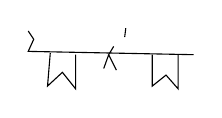
\begin{tikzpicture}[scale=.7]
\draw (0,.25)--(.1,.1)--(0,-.12)--(3,-.18);
\draw (.4,-.15)--(.35,-.75)--(.62,-.5)--(.86,-.8)--(.86,-.18);
\draw (2.25,-.18)--(2.25,-.75)--(2.5,-.55)--(2.72,-.8)--(2.72,-.18);
\draw (1.46,-.18)--(1.37,-.43) (1.46,-.18)--(1.6,-.46) (1.46,-.18)--(1.55,-.03);
\draw (1.75,.14)--(1.77,.3);
\end{tikzpicture}}

\deleted{\[
\boxed{G,\quad g_1,\qquad,\ g_r}
\]
\figure{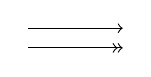
\begin{tikzpicture}\draw[->] (0,.25)--(1.2,.25);\draw[->>] (0,0)--(1.2,0);\end{tikzpicture}}
Diagramme de Cayley
\figure{\begin{tikzpicture}[scale=.9]
\coordinate (x) at (0,0);\coordinate (a) at (.1,1.2);\coordinate (b) at (1.65,1.18);
\draw (x)..controls (1.5,.8) and (4.4,1.1)..(3.9,2.1)..controls (3.3,3.2) and (.4,3.2)..(a);
\draw[->] (x)--(0.05,.62)--(a);\draw (x)..controls(-.1,.6)and(.05,.9)..(a);
\draw[->>] (a)--(.8,1.4);
\draw[->>] (x)--(.45,-.4);
\draw[->>] (x)--(.6,.38);\draw (.6,.38)--(b);
\fill (x) circle(1.6pt);\fill (a) circle(1.6pt);\fill (b) circle(1.4pt);
\node[below left] at(x){$x$};\node[below right] at(b){$xg_i$};
\fill (1.7,0) circle(1.1pt);\fill (3.4,0) circle(1.3pt);\fill (-1.6,.04) circle(1.1pt);\fill (-1.5,-.35) circle(1.1pt);
\draw (5.5,-.4)..controls(7.7,-.2)and(8.8,.2)..(8.3,1.4);
\node[below] at(5.5,-.4){$g$};\draw[->] (5.3,.15)..controls(5.3,-.1)..(5.5,-.25);
\end{tikzpicture}}
Mot \unsure{en les} $g_i$ $+$ origine
\[
g,\ g_i
\]}
\mspage{36}
\scanpage{38}
\margin{-- 180 --}
\margin{IX}
\uline{En d'autres termes, la filtration de} $\mathcal E^t$ \uline{induite par la filtration de Hodge} (\uline{avec les conventions de degrés} (13.4.6)) \uline{est concentrée en degré} $-1$, \uline{celle de} $\mathcal E/\mathcal E^f$ \uline{induite par la filtration de Hodge est concentrée en degré} $0$.

c) \uline{Considérons la filtration de}
\[
\mathcal E^{ab}\overset{\mathrm{dfn}}=\mathcal E^f/\mathcal E^t\simeq(\uline{\unsure{R}}^{ab})\otimes_{\mathbb Z}\uline{O}_S,\quad\text{où }\uline{R}^{ab}=\uline{R}^f/\uline{R}^t\quad(\text{cf. a)}),
\]
\figure{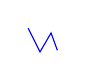
\begin{tikzpicture}\draw[blue] (0,.3)--(.15,0)--(.29,.24)--(.37,.02);\end{tikzpicture}}
\uline{induite par la filtration de Hodge de} $\mathcal E$,\uline{donc} \uline{définie par le sous-Module} $\uline{F}^{ab}$ \uline{de} $\mathcal E^{ab}$ \uline{image de}
\[
\uline{F}^f\overset{\mathrm{dfn}}=\uline{F}\cap\mathcal E^f\longrightarrow\mathcal E^{ab},
\]
\uline{(la flèche étant un monomorphisme grâce à la première relation} $(*)$).
\uline{Alors le couple} $(\uline{R}^{ab},\uline{F}^{ab}\subset\uline{R}^{ab}\otimes_{\mathbb Z}\uline{O}_S=\mathcal E^{ab})$ \uline{est isomorphe au couple} $(\uline{R}(B),\uline{F}(B))$ \uline{associé à un} groupe abéloïde \uline{sur} $S$, \uline{comme expliqué après} (13.4.4) (\uline{où donc} $B\simeq\mathcal E^{ab}/(F^{ab}+R^{ab})$, \uline{les symboles non soulignés désignant les groupes analytiques sur} $S$ \uline{correspondants}).

\uline{Remarque} 13.4.18. Dans la terminologie de DELIGNE [4], la conclusion de la proposition précédente, lorsqu'on se restreint au-dessus d'un ouvert $U$ de $S$ sur lequel $R$ est localement constant, exprime que $R$, muni des deux filtrations (13.4.17.1) de $\mathcal E=\uline{R}\otimes_{\mathbb Z}\uline{O}_S$, est une ``famille analytique de structures de Hodge mixtes sur $U$''. La situation qu'on vient d'expliciter a servie de modèle aux conjectures de DELIGNE sur la théorie de Néron en dimensions supérieures, énoncées dans [9, 9.8 à 9.13]. Il y a cependant un trait important de la théorie algébrique

\margin{498}
\fbox{498}
\mspage{37}
\scanpage{39}
\uline{\unsure{a'}}
\[
\operatorname{Hom}^d(M^*,\deleted{\unsure{\otimes_k}}N\otimes_k S_k)\simeq\operatorname{Hom}^d(\tau_{N-d}M,\tau_N(N\otimes_k S_k)
\]
\figure{\begin{tikzpicture}\draw (0,0)--(0,1);\draw (.1,1.05)--(8,1.05);\draw (.1,-.05)--(7.7,-.05);\end{tikzpicture}}
si $\left\{\begin{array}{l}M^*\in\mathcal M_{-d}\\N\geq0\end{array}\right.$

p. ex.
\diagram{\begin{tikzcd}[column sep=small]
\operatorname{Hom}^d(M\otimes_k S_k,N\otimes_k S_k) \arrow[r,"\sim"] \arrow[d,phantom,"\wr"] & \operatorname{Hom}^d(\tau_{N-d}M_{S_k},\tau_N N_{S_k} \\
\operatorname{Hom}^{\deleted{\unsure{d}}}_k(M,N) & \text{\uuline{si $d\geq0$}, $N\geq0$}
\end{tikzcd}}
\figure{\begin{tikzpicture}\draw (0,0)--(0,1);\draw (.2,1.1)--(8,1.1);\draw (.3,-.1)--(7.8,-.1);\end{tikzpicture}}

\unsure{Hom. hom} de degré $d\in\mathbb Z$
\diagram{\begin{tikzcd}
\tau_\alpha M_{S_k}\arrow[r] & \tau_\beta N_{S_k}
\end{tikzcd}} $(\beta\geq\alpha)$

a) \deleted{$d\geq0$}. Supposons d'abord $\boxed{d\geq\beta-\alpha}$ i.e $\alpha+d\geq\beta$

On a \deleted{$\unsure{\operatorname{Hom}^i(M)}$} --
\[
\operatorname{Hom}^d(\tau_\alpha M_{S_k},\tau_\beta N_{S_k})\overset{\sim}{\longleftrightarrow}\operatorname{Hom}^d(\tau_\alpha M_{S_k},\underbrace{\tau_{\unsure{\alpha+i|\alpha+d}}\tau_\beta N_{S_k}}_{=\tau_{\alpha+d}N_{S_k}})
\]
\[
\overset{\sim}{\longleftarrow}\operatorname{Hom}^d(M_{S_k},N_{S_k})\simeq\operatorname{Hom}_k(M,N)
\]
(si $u:M-N$, il lui correspond l'hom
\[
\underset{j\geq\alpha}{mT^{(j)}}\longmapsto u(m)T^{(d)}T^{(j)}=c_{d,j}u(m)T^{(d+j)}
\]
)

b) Supposons $0\leq d<\beta-\alpha$ \inserted{$\unsure{\text{i.e.}}\ \beta\geq\beta-d\unsure{>|\geq}\alpha$} on a alors
\deleted{\diagram{\begin{tikzcd}[column sep=small]
\operatorname{Hom}^d(\tau_\alpha M_{S_k},\tau_\beta N_{S_k})\arrow[r,"\unsure{\mathrm{res.}}"'] & \operatorname{Hom}^d(\tau_{\beta-d}M_{S_k},\tau_\beta N_{S_k})\arrow[d,phantom,"\wr"]\\
& \operatorname{Hom}_k(M,N)
\end{tikzcd}}}
\mspage{38}
\scanpage{40}
\margin{. 7 .}
$\circ$ \uline{Matériel commandé par Mme LATOUR} .

Mme LATOUR a commandé par simple lettre, en prévision de l'attribution d'un contrat de recherche, un caisson climatique sur mesure et un enregistreur, fourni il y a deux ans par la SECASI, non réglé à ce jour.

Mme LATOUR n'était aucunement habilitée à passer cette commande. Le Conseil Scientifique pense que l'Université n'est nullement engagée par cette commande tout à fait irrégulière. Le Président fait remarquer que l'Université est obligée de payer car ce matériel, bien que toujours en caisse, a été reçu à l'U.S.T.L. depuis 2 ans, et que toutes les tentatives pour le faire reprendre par le fournisseur sont demeurées vaines.

Il propose de récupérer , sur une période de 5 ans, le montant de la commande, sur les points chercheurs qui concernent Mme LATOUR.

Le Conseil Scientifique donne son accord sur cette procédure.

.VIII. \uuline{EXAMEN DE LA PROPOSITION DE M. MORET}
\margin{$\unsure{\longleftarrow}$}

( voir Page 4 du procès-verbal du Conseil Scientifique du 21 Mars 1975)

a) \uline{Modification des fiches chercheurs}

Après discussion,M. SIAU signale qu'une fiche est déjà établie pour chaque Maître Assistant en vue de l'avancement au choix. Si le Conseil Scientifique le désire, il peut avoir communication de ces fiches.

b) \uline{Répertoire des chercheurs qui ne publient pas depuis plusieurs années}

Ce travail sera confié à la Commission chargée d'étudier les rapports d'activité scientifique déjà parus (P.5 du procès verbal du 21 Mars dernier).
\figure{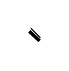
\begin{tikzpicture}\draw[very thick] (0,.12)--(.13,0);\draw (.02,.16)--(.14,.04);\end{tikzpicture}}

c) \uline{Publication nominative de toutes les heures supplémentaires}

Le Président \unsure{ROUZAUD} signale qu'il est très attentif au nombre d'heures supplémentaires attribuées à chaque enseignant de l'USTL, mais ne peut vérifier les heures supplémentaires assurées pour des organismes privés.
\figure{\begin{tikzpicture}\draw[very thick] (0,0)--(.14,.04)--(.23,.1);\end{tikzpicture}}

M. VIERNE souhaiterait qu'une information plus large sur les services assurés par les enseignants soit donnée.

Le Président ROUZAUD pense que le tableau des services pourrait être porté sur les tableaux d'affichage des commissions de spécialistes.
\mspage{39}
\scanpage{41}
\diagram{\begin{tikzcd}[column sep=small,row sep=large]
\operatorname{Hom}^d(\tau_\alpha M_{S_k},\underset{\substack{\cap\\\tau_{\alpha+d}N_{S_k}}}{\tau_\beta N_{S_k}})\arrow[r,hook] & \operatorname{Hom}^d(\tau_\alpha M_{S_k},\tau_{\alpha+d}N_{S_k})\arrow[d,phantom,"\wr"]\\
& \operatorname{Hom}_k(M,N)
\end{tikzcd}}
\margin{(sous-module des hom de degré $d$ de $\tau_\alpha M_{S_k}$ ds $\tau_{\alpha+d}N_{S_k}$ qui veulent bien appliquer $\tau_\alpha M_{S_k}$ dans $\tau_\beta N_{S_k}\subset\tau_{\alpha+d}N_{S_k}$)}

Il faut donc prendre un $u:M\longrightarrow N$ tel que l'hom correspondant $\tau_\alpha M_{S_k}-\tau_{\alpha+d}N_{S_k}$
\[
mT^{(j)}\longmapsto c_{dj}u(m)T^{(d+j)}
\]
\deleted{\unsure{applique} $M_S$} a son image dans $\tau_\beta\unsure{M|N}_{S_k}$, i.e. tel que
\[
\left\{\begin{array}{l}
c_{d,\alpha}u=0\\
c_{d,\alpha+1}u=0\\
\cdots\\
c_{d,\beta-d}u=0
\end{array}\right.
\]
(ce qui s'écrit
\[
c_{d,j}u=0\quad\text{si}\quad\alpha\leq j<\beta-d\quad\deleted{\unsure{\beta-d+1}}
\]
)

c) \uline{$d<0$}. Notons que
\[
\unsure{N^*_{\otimes S_k}|N^*_{S_k}}=\varphi_{0\beta}\tau_\beta N_{S_k}=\underset{\substack{\cap\\\varphi_\beta N_{S_k}}}{\tau_0\varphi_\beta\tau_\beta N_{S_k}}
\]
donc \inserted{si $M^*\in\operatorname{Ob}\mathcal M^*$}
\[
\begin{array}{ll}
\operatorname{Hom}^d(M^*,N_{S_k})\subset & \operatorname{Hom}^d(M^*,\varphi_\beta\tau_\beta N_{S_k})\\
& \Vert\\
& \operatorname{Hom}(M^{\unsure{*|\prime}}[-d],\varphi_\beta N_{S_k})\\
& \Vert\\
& \operatorname{Hom}(\tau_\beta M^{\unsure{*|\prime}}[-d],N_{S_k}
\end{array}
\]
\mspage{40}
\scanpage{42}
\margin{. \unsure{6|0} .}
Le Conseil Scientifique décide de répondre par la négative étant donné que la succession d'un laboratoire suppose l'acceptation de l'actif et du passif et que le reliquat 1973 laissé par Mle TUZET s'élevait à 18.956 F 23.

$\circ$ \uline{Demande de M. MATTAUER}

M. MATTAUER fait état d'un appareil de son laboratoire endommagé à la suite du branchement d'eau en 1973. En l'absence d'information plus complète, le Conseil Scientique surseoit à l'examen de cette demande.

Un rapport plus détaillé sera demandé à l'intéressé.

$\circ$ \uline{Demande de M.M. MATTAUER et LOUIS}

Demande de subvention pour couvrir les frais d'impression de la troisième réunion des Sciences de la Terre (23,24 et 25 avril 1975, à l'U.S.T.L.) qui s'élève à 9.313 F 96.

Cette subvention est accordée.

$\circ$ \uline{Demande de M. MORETTI}

19.000 F pour faire réparer un analyseur d'acides aminés. Le Conseil Scientifique fait remarquer que cet appareil servant aux T.P. de maîtrise, la demande doit être transmise au Directeur de l'U.E.R. de T.P. concerné.
\figure{\begin{tikzpicture}\draw[thick] (0,.15)--(.04,.05)--(.04,0);\end{tikzpicture}}

$\circ$ \uline{Demande de M. MATHIEU}

Brevet d'invention destiné à la S.N.C.F. Le Conseil Scientifique pense que cette demande ne rentre pas dans le cadre de ses attributions, bien que l'intérêt du travail de M. MATHIEU soit indiscutable.
\figure{\begin{tikzpicture}\draw[very thick] (0,0)--(.13,.02);\end{tikzpicture}}

$\circ$ \uline{Demande de M. AVEROUS}

Aide spéciale en vue de l'achat d'une microsonde électronique CAMECA au prix de 250.000 F après remise en état complète
\diagram{\begin{array}{ll}
\text{Participation C.N.R.S.}&\text{50.000 F}\\
\text{Participation Utilisateur}&\text{120.000 F}\\
\left.\begin{array}{l}\text{Participation demandée au}\\\text{Conseil Scientifique}\end{array}\right\}&\text{80.000 F}
\end{array}}

A la demande de M. MORET, M. PISTOULET donne quelques explications sur cet appareil. Le Conseil Scientifique accorde le crédit de 80.000 F demandé étant entendu que cet appareil sera installé en service commun, et fixe un délai maximal de 6 mois pour la mise en place de ce service microsonde.

$\circ$ \uline{Demande de M.M. IMBACH et JACQUIER}

Demande de 4.000 F pour l'organisation des 11èmes Rencontres de Chimie Thérapeutiques, les 10, 11 et 12 Septembre 1975.

Demande acceptée.
\mspage{41}
\scanpage{43}
$T_r\quad(=T^{(p^r)})$
\margin{\figure{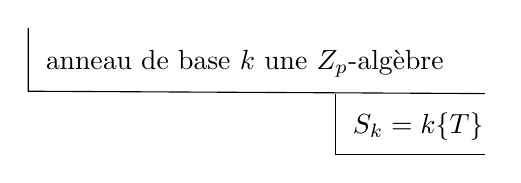
\begin{tikzpicture}[x=1cm,y=1cm]\node[anchor=west] at (.1,.35) {anneau de base $k$ une $\mathbb Z_p$-algèbre};\draw (0,.8)--(0,0)--(5.8,-.03);\node[anchor=west] at (4,-.45) {$S_k=k\{T\}$};\draw (3.9,-.03)--(3.9,-.8)--(5.8,-.8);\end{tikzpicture}}}
\[
T_r^p=p!(T^{(p^r)})^{(p)}=p!\underset{\substack{\Vert\\\frac{p^{r+1}!}{(p^r!)^p p!}\in\mathbb Z_p^*}}{\nu_r}T^{(p^{r+1})}=p\nu'_rT_{r+1}
\]
\[
\nu'_r=(p-1)!\frac{p^{r+1}!}{(p^r!)^p p!}\in\mathbb Z_p^*
\]
\[
\boxed{T_r^p=p\underset{\substack{\cap\\\mathbb Z_p^*}}{\nu'_r}T_{r+1}}
\]
$\tau_{p^r}S_k$ a comme base les $T_{\unsure{\bullet|*}}^{\uline{i}}$, $\uline{i}=(i_0,i_1,\cdots,i_r,i_{r+1},\cdots$
\[
\text{où}\quad\sum i_\alpha p^\alpha\geq p^r\quad\text{i.e.}\quad\exists\alpha\geq r\ \text{avec}\ i_\alpha\ne0
\]
Donc $\tau_{p^r}S$ est engendré par $\underset{\substack{\Vert\\t_r}}{T_r},\underset{\substack{\Vert\\t_{r+1}}}{T_{r+1}},\cdots,\underset{\ell\geq0}{T_{r+\ell}},\cdots$

les relations sont
\[
\boxed{T_s^{p-1}t_s=p\nu'_s t_{s+1}\qquad\text{si }s\geq r}.
\]
donc un hom de degré $d<p^r$, $d=d_0+d_1p\cdots+d_{r-1}p^{r-1}$
\diagram{\begin{tikzcd}
u:\tau_{p^r}S_k\arrow[r] & \unsure{M|N}\otimes_k S_k
\end{tikzcd}}
est donné par \unsure{des}
\[
\deleted{(\unsure{R_s})}\qquad\boxed{u(t_s)=\deleted{\unsure{\xi_s}T^{(p^s-d)}}\eta_s\in S_{\unsure{k}}^{(p^s-d)}\otimes_k M}
\]
avec les relations
\[
(R_s)\qquad\boxed{T_s^{p-1}\eta_s=p\nu'_s\eta_{s+1}}
\]
Soit $\nu=\unsure{\nu_p|v_p}(d)$ de sorte que
\[
d=d_\nu p^\nu\cdots+d_{r-1}p^{r-1}=p^\nu(d_\nu+d_{\nu+1}p\cdots+d_{r-1}p^{r-1-\nu}
\]
$d_\nu\ne0$ i.e. $d_\nu\geq1$
\[
p^s-d=p^\nu\left(p^{s-\nu}-\frac d{p^\nu}\right)=p^\nu\left(p^{s-\nu}-1-\underbrace{\left(\frac d{p^\nu}-1\right)}_{(d_\nu-1)+d_{\nu+1}p\cdots+d_{r-1}p^{r-1-\nu}}\right.
\]
\[
=p^\nu\left(\underset{\substack{\Vert\\(p-1)-(d_\nu-1)}}{\delta_\nu}+\underset{\substack{\Vert\\(p-1)-d_{\nu+1}}}{\delta_{\nu+1}}p\cdots+\underset{\substack{\Vert\\(p-1)-(d_{r-1})}}{\delta_{r-1}}p^{r-\nu-1}+\underbrace{(p-1)p^{r-\nu}+(p-1)p^{r-\nu+1}+\cdots+(p-1)p^{s-\nu-1}}_{\text{si }s>r}\right.
\]
donc $S^{(p^s-d)}$ a comme base
\[
\deleted{\unsure{T_\beta}}T_\nu^{\delta_\nu}T_{\nu+1}^{\delta_{\nu+1}}\cdots T_{r-1}^{\delta_{r-1}}(T_r^{\deleted{\unsure{p-1}}}\cdots T_{s-1})^{p-1}
\]
\margin{$\longrightarrow$ à facteur \unsure{inv. près} si $s>r$}
\mspage{42}
\scanpage{44}
\margin{. 2 .}
\uuline{O R D R E\qquad D U\qquad J O U R}

.I. \uuline{APPROBATION DU DERNIER PROCES VERBAL} (21.03.1975)

Aucune observation n'étant faite, ce procès-verbal est approuvé à l'unanimité.

.II. \uuline{EXAMEN DE LA SITUATION DES MAITRES DE CONFERENCES NOMMES EN SURNOMBRE}

Auparavant chaque Maître de Conférences nouvellement nommé touchait, en plus de la part fixe de crédit recherche, un forfait de 15 points chercheurs pendant 2 ans, ce qui permettait au nouveau laboratoire de démarrer et lui donnait le temps de former une équipe de chercheurs. Ce phénomène s'est généralisé à tous les nouveaux nommés.
M. PISTOULET fait remarquer que c'est une prime supplémentaire donnée aux Maîtres de Conférences nommés en surnombre qui ne forment pas une nouvelle équipe de recherche, mais travaillent au sein d'un laboratoire déjà constitué.
\figure{\begin{tikzpicture}\draw (0,0)--(.03,.15)--(.09,.04)--(.17,.13);\draw (.03,.06)--(.15,.05);\end{tikzpicture}}

Le Président ROUZAUD signale que dans les 3 ou 4 années à venir, de nombreux retours sont prévus.

Après discussion, le Conseil Scientifique décide qu'il n'est plus possible d'accorder le bénéfice des 15 points aux Maîtres de Conférences ou Professeurs nommés en surnombre. Cette règle sera maintenue pour les Maîtres de Conférences déjà en place en 1975. Les derniers 15 points \unsure{dîts|dits} ``JEUNES LABOS'' seront donc distribués en 1975.

.III. \uuline{EXAMEN DES CAS PARTICULIERS - RAPPORT DE LA COMMISSION CHERCHEURS}

M. GAUFRES, Secrétaire de la Commission chargée de l'examen des cas particuliers, expose et commente le rapport : après discussion ce rapport est adopté, une phrase ayant été ajoutée à la fin des paragraphes a) et b) de la 2ème partie.

(voir texte en annexe)

En ce qui concerne les cas précis :

\uline{Cas de Mme MALEVILLE} : La Commission demande que l'intéressée fasse la preuve de son activité scientifique (publications).

\uline{Cas des Chercheurs de M. ESCOUFFIER} : M. PISTOULET lit la lettre de M. ESCOUFFIER mais son problème est résolu par le paragraphe 1 du rapport de la Commission.
\mspage{43}
\scanpage{45}
On pourra donc poser
\[
\eta_s=\xi_s T_\nu^{\delta_\nu}T_{\nu+1}^{\delta_{\nu+1}}\cdots T_{r-1}^{\delta_{r-1}}(T_r,\cdots T_{s-1})^{p-1}
\]
avec $\xi_s\in M$

On aura
\[
\eta_sT_s^{p-1}=\xi_sT_\nu^{\delta_\nu}\cdots T_{r-1}^{\delta_{r-1}}(T_r\cdots T_s)^{p-1}
\]
Et relation $(R_s)$ s'écrit donc, comme
\[
p\nu'_s\eta_{s+1}=\unsure{(p\nu'_s)}\xi_{s+1}T_\nu^{\delta_\nu}\cdots T_{r-1}^{\delta_{r-1}}(T_r\cdots T_s)^{p-1}
\]
\[
\boxed{\xi_s=p\nu'_s\xi_{s+1}}
\]
On aura donc
\[
\xi_s=p^h\nu'_s\cdots\nu'_{s+h-1}\xi_{s+h}\qquad\forall h\geq1
\]
donc
\[
\xi_s\in\deleted{\unsure{\varphi}}\bigcap_h(p^hM)
\]
i.e. les $\xi_s$ appartiennent à la partie divisible de $\uline{M}$.
\figure{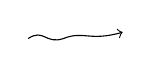
\begin{tikzpicture}\draw[->] (0,0)..controls(.2,.13)and(.22,-.08)..(.45,0)..controls(.7,.1)and(.78,-.04)..(1.2,.08);\end{tikzpicture}}

\uline{Prop} Soit $k$ un anneau comm., $\unsure{S_k|B_k}=k\{T\}$, $M,N$ deux $k$-modules, avec $d>0$, $N_0^{\unsure{?|*}}=\bigcap_{n\in\mathbb N^*}nN$ le \deleted{partie} \inserted{plus grand sous-module} divisible de $N$, $\alpha\geq d$. Alors si $u\in\operatorname{Hom}^{-d}(\tau_\alpha M_{S_k},N_{S_k})$ (\deleted{qui} \inserted{lequel module} est indépendant \unsure{mod variation} du choix de $\alpha$), $u$ se factorise par $N_{0S_k}$, i.e.
\[
\operatorname{Hom}^{-d}(\tau_\alpha M_{S_k},N_{S_k})\overset{\sim}{\longleftrightarrow}\operatorname{Hom}^{-d}(\tau_\alpha M_{S_k},N_{0S_k})
\]
\uline{Cor} Si $N_0=0$, p. ex. $k$ de torsion, alors $\operatorname{Hom}^{-d}(\tau_\alpha M_{S_k},N_{S_k})=0$
\mspage{44}
\scanpage{46}
\margin{-- 176 --}
\margin{IX}
un homomorphisme canonique
\[
(13.4.2)\qquad\mathcal E=\uline{R}\otimes_{\mathbb Z}\uline{O}_S\longrightarrow\uline{E},
\]
dont le noyau sera noté $\uline{F}(A)$ ou simplement $\uline{F}$, de sorte qu'on a une suite exacte

(13.4.3)\quad\diagram{\begin{tikzcd}
0\arrow[r]&\uline{F}\arrow[r]&\mathcal E\arrow[r]&\uline{E}
\end{tikzcd}}.

Le cas le plus intéressant est celui où l'homomorphisme (13.4.2) est un épimorphisme, i.e. où pour tout $s\in S$, $R_s$ engendre le vectoriel complexe $E_s$. Dans ce cas on trouve donc une suite exacte

(13.4.4)\quad\diagram{\begin{tikzcd}
0\arrow[r]&\uline{F}\arrow[r]&\mathcal E\arrow[r]&\uline{E}\arrow[r]&0
\end{tikzcd}},

et si $R$ est localement constant, c'est là une suite exacte courte de Modules localement libres sur $S$. La connaissance du couple $(E,R)$ est alors équivalente à celle du couple $(R,\uline{F})$, où $R$ est un groupe analytique localement constant sur $S$ à fibres des $\mathbb Z$-Modules libres de type fini, et $\uline{F}$ est un sous-Module localement facteur direct de $\mathcal E=\uline{R}\otimes_{\mathbb Z}\uline{O}_S$, tel que l'on ait de plus la relation
\[
(13.4.5)\qquad\uline{F}\cap\uline{R}=0.
\]
Du point de vue des structures de Hodge, il y a lieu de regarder $\mathcal E$ comme filtré par la ``\uline{filtration de Hodge}''
\[
(13.4.6)\qquad\operatorname{Fil}^1(\mathcal E)=\mathcal E,\quad\operatorname{Fil}^0(\mathcal E)=\uline{F},\quad\operatorname{Fil}^{-1}(\mathcal E)=0.
\]
Notons que la suite exacte (13.4.3) dépend encore fonctoriellement du groupe analytique $A$ sur $S$, et qu'elle commute aux changements de base quelconques.
\figure{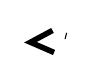
\begin{tikzpicture}\draw[line width=2pt] (.28,.15)--(0,0)--(.3,-.13);\draw (.46,.12)--(.44,.04);\end{tikzpicture}}
\margin{494}
\fbox{494}
\mspage{45}
